% BEGIN CLASS DEPENDENCIES
\begin{filecontents*}{iopart.cls}
%% 
%% This is file `iopart.cls'
%% 
%% This file is distributed in the hope that it will be useful, 
%% but WITHOUT ANY WARRANTY; without even the implied warranty of 
%% MERCHANTABILITY or FITNESS FOR A PARTICULAR PURPOSE. 
%% 
%% Licensed under the LPPL: http://www.latex-project.org/lppl.txt
%% Current Maintainer: IOP Publishing Ltd
%% 
%% \CharacterTable
%%  {Upper-case    \A\B\C\D\E\F\G\H\I\J\K\L\M\N\O\P\Q\R\S\T\U\V\W\X\Y\Z
%%   Lower-case    \a\b\c\d\e\f\g\h\i\j\k\l\m\n\o\p\q\r\s\t\u\v\w\x\y\z
%%   Digits        \0\1\2\3\4\5\6\7\8\9
%%   Exclamation   \!     Double quote  \"     Hash (number) \#
%%   Dollar        \$     Percent       \%     Ampersand     \&
%%   Acute accent  \'     Left paren    \(     Right paren   \)
%%   Asterisk      \*     Plus          \+     Comma         \,
%%   Minus         \-     Point         \.     Solidus       \/
%%   Colon         \:     Semicolon     \;     Less than     \<
%%   Equals        \=     Greater than  \>     Question mark \?
%%   Commercial at \@     Left bracket  \[     Backslash     \\
%%   Right bracket \]     Circumflex    \^     Underscore    \_
%%   Grave accent  \`     Left brace    \{     Vertical bar  \|
%%   Right brace   \}     Tilde         \~}
%
\NeedsTeXFormat{LaTeX2e}
\ProvidesClass{iopart}[1996/06/10 v0.0 IOP Journals LaTeX article class]
\newcommand\@ptsize{0}
\newif\if@restonecol
\newif\if@titlepage
\newif\ifiopams
\@titlepagefalse
\DeclareOption{a4paper}
   {\setlength\paperheight {297mm}%
    \setlength\paperwidth  {210mm}}
\DeclareOption{letterpaper}
   {\setlength\paperheight {11in}%
    \setlength\paperwidth  {8.5in}}
\DeclareOption{landscape}
   {\setlength\@tempdima   {\paperheight}%
    \setlength\paperheight {\paperwidth}%
    \setlength\paperwidth  {\@tempdima}}
\DeclareOption{10pt}{\renewcommand\@ptsize{0}}
\DeclareOption{11pt}{\renewcommand\@ptsize{2}} % No 11pt version
\DeclareOption{12pt}{\renewcommand\@ptsize{2}}
\DeclareOption{draft}{\setlength\overfullrule{5pt}}
\DeclareOption{final}{\setlength\overfullrule{0pt}}
\DeclareOption{titlepage}{\@titlepagetrue}
\DeclareOption{notitlepage}{\@titlepagefalse}
\ExecuteOptions{letterpaper,final}
\ProcessOptions
\DeclareMathAlphabet{\bi}{OML}{cmm}{b}{it}
\DeclareMathAlphabet{\bcal}{OMS}{cmsy}{b}{n}
\input{iopart1\@ptsize.clo}
\setlength\lineskip{1\p@}
\setlength\normallineskip{1\p@}
\renewcommand\baselinestretch{}
\setlength\parskip{0\p@ \@plus \p@}
\@lowpenalty   51
\@medpenalty  151
\@highpenalty 301
\setlength\parindent{2em}
\setcounter{topnumber}{8}
\renewcommand\topfraction{1}
\setcounter{bottomnumber}{3}
\renewcommand\bottomfraction{.99}
\setcounter{totalnumber}{8}
\renewcommand\textfraction{0.01}
\renewcommand\floatpagefraction{.8}
\setcounter{dbltopnumber}{6}
\renewcommand\dbltopfraction{1}
\renewcommand\dblfloatpagefraction{.8}
%
\pretolerance=5000
\tolerance=8000
%
% Headings for all pages apart from first
%
\def\ps@headings{\let\@oddfoot\@empty
      \let\@evenfoot\@empty
      \def\@evenhead{\thepage\hfil\itshape\rightmark}%
      \def\@oddhead{{\itshape\leftmark}\hfil\thepage}%
      \let\@mkboth\markboth
      \let\sectionmark\@gobble
      \let\subsectionmark\@gobble}
%
% Headings for first page
%
\def\ps@myheadings{\let\@oddfoot\@empty\let\@evenfoot\@empty
    \let\@oddhead\@empty\let\@evenhead\@empty
    \let\@mkboth\@gobbletwo
    \let\sectionmark\@gobble
    \let\subsectionmark\@gobble}
%
% \maketitle just ends page
%
\newcommand\maketitle{\newpage}
%
% Article titles
%
% Usage: \title[Short title]{Full title}
% [Short title] is optional; use where title is too long
% or contains footnotes, 50 characters maximum 
%
\renewcommand{\title}{\@ifnextchar[{\@stitle}{\@ftitle}}
\def\@stitle[#1]#2{\markboth{#1}{#1}%
    \thispagestyle{myheadings}%
    \vspace*{3pc}{\exhyphenpenalty=10000\hyphenpenalty=10000 
    \Large\raggedright\noindent
    \bf#2\par}}
\def\@ftitle#1{\markboth{#1}{#1}%
    \thispagestyle{myheadings}%
    \vspace*{3pc}{\exhyphenpenalty=10000\hyphenpenalty=10000 
    \Large\raggedright\noindent
    \bf#1\par}}
%
% Can use \paper instead of \title
%
\let\paper=\title
%
% Generic title command for articles other than papers
%
% Usage: \article[Short title]{Article Type}{Full title}
% [Short title] is optional; use where title is too long
% or contains footnotes, 50 characters maximum 
%
\newcommand{\article}{\@ifnextchar[{\@sarticle}{\@farticle}}
\def\@sarticle[#1]#2#3{\markboth{#1}{#1}%
    \thispagestyle{myheadings}%
     \vspace*{.5pc}%
    {\parindent=\mathindent \bf #2\par}%
     \vspace*{1.5pc}%
    {\exhyphenpenalty=10000\hyphenpenalty=10000
     \Large\raggedright\noindent
     \bf#3\par}}%
\def\@farticle#1#2{\markboth{#2}{#2}%
    \thispagestyle{myheadings}%
     \vspace*{.5pc}%
    {\parindent=\mathindent \bf #1\par}%
     \vspace*{1.5pc}%
    {\exhyphenpenalty=10000\hyphenpenalty=10000
     \Large\raggedright\noindent
     \bf#2\par}}%
%
% Letters to the Editor
%
% Usage \letter{Full title}
% No short title is required for Letters
%
\def\letter#1{\article[Letter to the Editor]{Letter to the Editor}{#1}}
%
% Fast Track Communications (added by sxb 9 March 2011)
%
% Usage \ftc{Full title} - there's no short title
\def\ftc#1{\article[Fast Track Communication]{Fast Track Communication}{#1}}
%
%
% Review articles
%
% Usage: \review[Short title]{Full title}
% [Short title] is optional; use where title is too long
% or contains footnotes, 50 characters maximum 
%
\def\review{\@ifnextchar[{\@sreview}{\@freview}}
\def\@sreview[#1]#2{\@sarticle[#1]{Review Article}{#2}}
\def\@freview#1{\@farticle{Review Article}{#1}}
%
% Topical Review
%
% Usage: \topical[Short title]{Full title}
% [Short title] is optional; use where title is too long
% or contains footnotes, 50 characters maximum 
%
\def\topical{\@ifnextchar[{\@stopical}{\@ftopical}}
\def\@stopical[#1]#2{\@sarticle[#1]{Topical Review}{#2}}
\def\@ftopical#1{\@farticle{Topical Review}{#1}}
%
% Comments
%
% Usage: \comment[Short title]{Full title}
% [Short title] is optional; use where title is too long
% or contains footnotes, 50 characters maximum 
%
\def\comment{\@ifnextchar[{\@scomment}{\@fcomment}}
\def\@scomment[#1]#2{\@sarticle[#1]{Comment}{#2}}
\def\@fcomment#1{\@farticle{Comment}{#1}}
%
% Rapid Communications
%
% Usage: \rapid[Short title]{Full title}
% [Short title] is optional; use where title is too long
% or contains footnotes, 50 characters maximum 
%
\def\rapid{\@ifnextchar[{\@srapid}{\@frapid}}
\def\@srapid[#1]#2{\@sarticle[#1]{Rapid Communication}{#2}}
\def\@frapid#1{\@farticle{Rapid Communication}{#1}}
%
% Notes
%
% Usage: \note[Short title]{Full title}
% [Short title] is optional; use where title is too long
% or contains footnotes, 50 characters maximum 
%
\def\note{\@ifnextchar[{\@snote}{\@fnote}}
\def\@snote[#1]#2{\@sarticle[#1]{Note}{#2}}
\def\@fnote#1{\@farticle{Note}{#1}}
%
% Preliminary Communications
%
% Usage: \prelim[Short title]{Full title}
% [Short title] is optional; use where title is too long
% or contains footnotes, 50 characters maximum 
%
\def\prelim{\@ifnextchar[{\@sprelim}{\@fprelim}}
\def\@sprelim[#1]#2{\@sarticle[#1]{Preliminary Communication}{#2}}
\def\@fprelim#1{\@farticle{Preliminary Communication}{#1}}
%
% List of authors
%
% Usage \author[Short form]{List of all authors}
% The short form excludes footnote symbols linking authors to addresses 
% and is used for running heads in printed version (but not on preprints)
%
\renewcommand{\author}{\@ifnextchar[{\@sauthor}{\@fauthor}}
\def\@sauthor[#1]#2{\markright{#1}    % for production only
   \vspace*{1.5pc}%
   \begin{indented}%
   \item[]\normalsize\bf\raggedright#2
   \end{indented}%
   \smallskip}
\def\@fauthor#1{%\markright{#1}         for production only
   \vspace*{1.5pc}%
   \begin{indented}%
   \item[]\normalsize\bf\raggedright#1
   \end{indented}%
   \smallskip}
%
% Affiliation (authors address)
%
% Usage: \address{Address of first author}
%        \address{Address of second author}
% Use once for each address, use symbols \dag \ddag \S \P $\|$
% to connect authors with addresses
%
\newcommand{\address}[1]{\begin{indented}
   \item[]\rm\raggedright #1
   \end{indented}}
%
% American Mathematical Society Classification Numbers
% Usage: \ams{57.XX, 58.XX}
%
\def\ams#1{\vspace{10pt}
     \begin{indented}
     \item[]\rm AMS classification scheme numbers: #1\par
     \end{indented}}
%
% A single Physics & Astronomy Classification Number
% Usage \pacno{31.10}
%
\def\pacno#1{\vspace{10pt}
     \begin{indented}
     \item[]\rm PACS number: #1\par
     \end{indented}}
%
% Physics & Astronomy Classification Numbers (more than one)
% Usage \pacs{31.10, 31.20T}
%
\def\pacs#1{\vspace{10pt}
     \begin{indented}
     \item[]\rm PACS numbers: #1\par
     \end{indented}}
%
% Submission details. If \jl command used journals name printed
% otherwise Institute of Physics Publishing 
%
\def\submitted{\vspace{28pt plus 10pt minus 18pt}
     \noindent{\small\rm Submitted to: {\it \journal}\par}}
%
\def\submitto#1{\vspace{28pt plus 10pt minus 18pt}
     \noindent{\small\rm Submitted to: {\it #1}\par}}
%
% For articles (other than Letters) not divided into sections
% Usage \nosections Start of text
%
\def\nosections{\vspace{30\p@ plus12\p@ minus12\p@}
    \noindent\ignorespaces}
%
% Acknowledgments (no heading if letter)
% Usage \ack for Acknowledgments, \ackn for Acknowledgement
%
\def\ack{\ifletter\bigskip\noindent\ignorespaces\else
    \section*{Acknowledgments}\fi}
\def\ackn{\ifletter\bigskip\noindent\ignorespaces\else
    \section*{Acknowledgment}\fi}
%
% Footnotes: symbols selected in order \dag (1), \ddag (2), \S (3), 
% $\|$ (4), $\P$ (5), $^+$ (6), $^*$ (7), \sharp (8), \dagger\dagger (9)
% unless optional argument of [<num>] use to specify required symbol, 
% 1=\dag, 2=\ddag, etc
% Usage: \footnote{Text of footnote}
%        \footnote[3]{Text of footnote}
%
\def\footnoterule{}%
\setcounter{footnote}{1}
\long\def\@makefntext#1{\parindent 1em\noindent 
 \makebox[1em][l]{\footnotesize\rm$\m@th{\fnsymbol{footnote}}$}%
 \footnotesize\rm #1}
\def\@makefnmark{\hbox{${\fnsymbol{footnote}}\m@th$}}
\def\@thefnmark{\fnsymbol{footnote}}
\def\footnote{\@ifnextchar[{\@xfootnote}{\stepcounter{\@mpfn}%
       \begingroup\let\protect\noexpand
       \xdef\@thefnmark{\thempfn}\endgroup
     \@footnotemark\@footnotetext}}
\def\@xfootnote[#1]{\setcounter{footnote}{#1}%
   \addtocounter{footnote}{-1}\footnote}
\def\@fnsymbol#1{\ifcase#1\or \dagger\or \ddagger\or \S\or
   \|\or \P\or ^{+}\or ^{\tsty *}\or \sharp
   \or \dagger\dagger \else\@ctrerr\fi\relax}
%
% IOP Journals
%
\newcounter{jnl}
\newcommand{\jl}[1]{\setcounter{jnl}{#1}}
\def\journal{\ifnum\thejnl=0 Institute of Physics Publishing\fi
        \ifnum\thejnl=1 J. Phys.\ A: Math.\ Gen.\ \fi
        \ifnum\thejnl=2 J. Phys.\ B: At.\ Mol.\ Opt.\ Phys.\ \fi
        \ifnum\thejnl=3 J. Phys.:\ Condens. Matter\ \fi
        \ifnum\thejnl=4 J. Phys.\ G: Nucl.\ Part.\ Phys.\ \fi
        \ifnum\thejnl=5 Inverse Problems\ \fi
        \ifnum\thejnl=6 Class. Quantum Grav.\ \fi
        \ifnum\thejnl=7 Network: Comput.\ Neural Syst.\ \fi
        \ifnum\thejnl=8 Nonlinearity\ \fi
        \ifnum\thejnl=9 J. Opt. B: Quantum Semiclass. Opt.\ \fi
        \ifnum\thejnl=10 Waves Random Media\ \fi
        \ifnum\thejnl=11 J. Opt. A: Pure Appl. Opt.\ \fi
        \ifnum\thejnl=12 Phys. Med. Biol.\ \fi
        \ifnum\thejnl=13 Modelling Simul.\ Mater.\ Sci.\ Eng.\ \fi
        \ifnum\thejnl=14 Plasma Phys. Control. Fusion\ \fi
        \ifnum\thejnl=15 Physiol. Meas.\ \fi
        \ifnum\thejnl=16 Combust. Theory Modelling\ \fi
        \ifnum\thejnl=17 High Perform.\ Polym.\ \fi
        \ifnum\thejnl=18 Public Understand. Sci.\ \fi
        \ifnum\thejnl=19 Rep.\ Prog.\ Phys.\ \fi
        \ifnum\thejnl=20 J.\ Phys.\ D: Appl.\ Phys.\ \fi
        \ifnum\thejnl=21 Supercond.\ Sci.\ Technol.\ \fi
        \ifnum\thejnl=22 Semicond.\ Sci.\ Technol.\ \fi
        \ifnum\thejnl=23 Nanotechnology\ \fi
        \ifnum\thejnl=24 Measur.\ Sci.\ Technol.\ \fi
        \ifnum\thejnl=25 Plasma.\ Sources\ Sci.\ Technol.\ \fi
        \ifnum\thejnl=26 Smart\ Mater.\ Struct.\ \fi
        \ifnum\thejnl=27 J.\ Micromech.\ Microeng.\ \fi
        \ifnum\thejnl=28 Distrib.\ Syst.\ Engng\ \fi
        \ifnum\thejnl=29 Bioimaging\ \fi
        \ifnum\thejnl=30 J.\ Radiol. Prot.\ \fi
        \ifnum\thejnl=31 Europ. J. Phys.\ \fi
        \ifnum\thejnl=32 J. Opt. A: Pure Appl. Opt.\ \fi
        \ifnum\thejnl=33 New. J. Phys.\ \fi}
%
% E-mail addresses (to provide links from headers)
%
\def\eads#1{\vspace*{5pt}\address{E-mail: #1}}
\def\ead#1{\vspace*{5pt}\address{E-mail: \mailto{#1}}}
\def\mailto#1{{\tt #1}}
%
% Switches
%
\newif\ifletter
%
\setcounter{secnumdepth}{3}
\newcounter {section}
\newcounter {subsection}[section]
\newcounter {subsubsection}[subsection]
\newcounter {paragraph}[subsubsection]
\newcounter {subparagraph}[paragraph]
\renewcommand\thesection       {\arabic{section}}
\renewcommand\thesubsection    {\thesection.\arabic{subsection}}
\renewcommand\thesubsubsection {\thesubsection.\arabic{subsubsection}}
\renewcommand\theparagraph     {\thesubsubsection.\arabic{paragraph}}
\renewcommand\thesubparagraph  {\theparagraph.\arabic{subparagraph}}
\def\@chapapp{Section}

\newcommand\section{\@startsection {section}{1}{\z@}%
                   {-3.5ex \@plus -1ex \@minus -.2ex}%
                   {2.3ex \@plus.2ex}%
                   {\reset@font\normalsize\bfseries\raggedright}}
\newcommand\subsection{\@startsection{subsection}{2}{\z@}%
                   {-3.25ex\@plus -1ex \@minus -.2ex}%
                   {1.5ex \@plus .2ex}%
                   {\reset@font\normalsize\itshape\raggedright}}
\newcommand\subsubsection{\@startsection{subsubsection}{3}{\z@}%
                                     {-3.25ex\@plus -1ex \@minus -.2ex}%
                                     {-1em \@plus .2em}%
                                     {\reset@font\normalsize\itshape}}
\newcommand\paragraph{\@startsection{paragraph}{4}{\z@}%
                                    {3.25ex \@plus1ex \@minus.2ex}%
                                    {-1em}%
                                    {\reset@font\normalsize\itshape}}
\newcommand\subparagraph{\@startsection{subparagraph}{5}{\parindent}%
                                       {3.25ex \@plus1ex \@minus .2ex}%
                                       {-1em}%
                                      {\reset@font\normalsize\itshape}}
\def\@sect#1#2#3#4#5#6[#7]#8{\ifnum #2>\c@secnumdepth
     \let\@svsec\@empty\else
     \refstepcounter{#1}\edef\@svsec{\csname the#1\endcsname. }\fi
     \@tempskipa #5\relax
      \ifdim \@tempskipa>\z@
        \begingroup #6\relax
          \noindent{\hskip #3\relax\@svsec}{\interlinepenalty \@M #8\par}%
        \endgroup
       \csname #1mark\endcsname{#7}\addcontentsline
         {toc}{#1}{\ifnum #2>\c@secnumdepth \else
                      \protect\numberline{\csname the#1\endcsname}\fi
                    #7}\else
        \def\@svsechd{#6\hskip #3\relax  %% \relax added 2 May 90
                   \@svsec #8\csname #1mark\endcsname
                      {#7}\addcontentsline
                           {toc}{#1}{\ifnum #2>\c@secnumdepth \else
                             \protect\numberline{\csname the#1\endcsname}\fi
                       #7}}\fi
     \@xsect{#5}}
%
\def\@ssect#1#2#3#4#5{\@tempskipa #3\relax
   \ifdim \@tempskipa>\z@
     \begingroup #4\noindent{\hskip #1}{\interlinepenalty \@M #5\par}\endgroup
   \else \def\@svsechd{#4\hskip #1\relax #5}\fi
    \@xsect{#3}}

\setlength\leftmargini{2em}
\setlength\leftmarginii{2em}
\setlength\leftmarginiii{1.8em}
\setlength\leftmarginiv{1.6em}
\setlength\leftmarginv{1em}
\setlength\leftmarginvi{1em}
\setlength\leftmargin{\leftmargini}
\setlength\labelsep{0.5em}
\setlength\labelwidth{\leftmargini}
\addtolength\labelwidth{-\labelsep}
\@beginparpenalty -\@lowpenalty
\@endparpenalty   -\@lowpenalty
\@itempenalty     -\@lowpenalty
\renewcommand\theenumi{\roman{enumi}}
\renewcommand\theenumii{\alph{enumii}}
\renewcommand\theenumiii{\arabic{enumiii}}
\renewcommand\theenumiv{\Alph{enumiv}}
\newcommand\labelenumi{(\theenumi)}
\newcommand\labelenumii{(\theenumii)}
\newcommand\labelenumiii{\theenumiii.}
\newcommand\labelenumiv{(\theenumiv)}
\renewcommand\p@enumii{(\theenumi)}
\renewcommand\p@enumiii{(\theenumi.\theenumii)}
\renewcommand\p@enumiv{(\theenumi.\theenumii.\theenumiii)}
\newcommand\labelitemi{$\m@th\bullet$}
\newcommand\labelitemii{\normalfont\bfseries --}
\newcommand\labelitemiii{$\m@th\ast$}
\newcommand\labelitemiv{$\m@th\cdot$}
\newenvironment{description}
               {\list{}{\labelwidth\z@ \itemindent-\leftmargin
                        \let\makelabel\descriptionlabel}}
               {\endlist}
\newcommand\descriptionlabel[1]{\hspace\labelsep
                                \normalfont\bfseries #1}
\newenvironment{abstract}{%
      \vspace{16pt plus3pt minus3pt}
      \begin{indented}
      \item[]{\bfseries \abstractname.}\quad\rm\ignorespaces} 
      {\end{indented}\if@titlepage\newpage\else\vspace{18\p@ plus18\p@}\fi}
\newenvironment{verse}
               {\let\\=\@centercr
                \list{}{\itemsep      \z@
                        \itemindent   -1.5em%
                        \listparindent\itemindent
                        \rightmargin  \leftmargin
                        \advance\leftmargin 1.5em}%
                \item[]}
               {\endlist}
\newenvironment{quotation}
               {\list{}{\listparindent 1.5em%
                        \itemindent    \listparindent
                        \rightmargin   \leftmargin
                        \parsep        \z@ \@plus\p@}%
                \item[]}
               {\endlist}
\newenvironment{quote}
               {\list{}{\rightmargin\leftmargin}%
                \item[]}
               {\endlist}
\newenvironment{titlepage}
    {%
        \@restonecolfalse\newpage
      \thispagestyle{empty}%
      \if@compatibility
        \setcounter{page}{0}
      \else
        \setcounter{page}{1}%
      \fi}%
    {\newpage\setcounter{page}{1}}
\def\appendix{\@ifnextchar*{\@appendixstar}{\@appendix}}
\def\@appendix{\eqnobysec\@appendixstar}
\def\@appendixstar{\@@par
 \ifnumbysec                         %  Added 30/4/94 to get Table A1,
 \@addtoreset{table}{section}        %  Table B1 etc if numbering by
 \@addtoreset{figure}{section}\fi    %  section
 \setcounter{section}{0}
 \setcounter{subsection}{0}
 \setcounter{subsubsection}{0}
 \setcounter{equation}{0}
 \setcounter{figure}{0}
 \setcounter{table}{0}
 \def\thesection{Appendix \Alph{section}}   
 \def\theequation{\ifnumbysec
      \Alph{section}.\arabic{equation}\else
      \Alph{section}\arabic{equation}\fi}  % Comment A\arabic{equation} maybe
 \def\thetable{\ifnumbysec                 % better? 15/4/95
      \Alph{section}\arabic{table}\else
      A\arabic{table}\fi}
 \def\thefigure{\ifnumbysec
      \Alph{section}\arabic{figure}\else
      A\arabic{figure}\fi}}
\def\noappendix{\setcounter{figure}{0}
     \setcounter{table}{0}
     \def\thetable{\arabic{table}}
     \def\thefigure{\arabic{figure}}}
\setlength\arraycolsep{5\p@}
\setlength\tabcolsep{6\p@}
\setlength\arrayrulewidth{.4\p@}
\setlength\doublerulesep{2\p@}
\setlength\tabbingsep{\labelsep}
\skip\@mpfootins = \skip\footins
\setlength\fboxsep{3\p@}
\setlength\fboxrule{.4\p@}
\renewcommand\theequation{\arabic{equation}}
\newcounter{figure}
\renewcommand\thefigure{\@arabic\c@figure}
\def\fps@figure{tbp}
\def\ftype@figure{1}
\def\ext@figure{lof}
\def\fnum@figure{\figurename~\thefigure}
\newenvironment{figure}{\footnotesize\rm\@float{figure}}%
    {\end@float\normalsize\rm}
\newenvironment{figure*}{\footnotesize\rm\@dblfloat{figure}}{\end@dblfloat}
\newcounter{table}
\renewcommand\thetable{\@arabic\c@table}
\def\fps@table{tbp}
\def\ftype@table{2}
\def\ext@table{lot}
\def\fnum@table{\tablename~\thetable}
\newenvironment{table}{\footnotesize\rm\@float{table}}%
   {\end@float\normalsize\rm}
\newenvironment{table*}{\footnotesize\rm\@dblfloat{table}}%
   {\end@dblfloat\normalsize\rm}
\newlength\abovecaptionskip
\newlength\belowcaptionskip
\setlength\abovecaptionskip{10\p@}
\setlength\belowcaptionskip{0\p@}
%
% Added redefinition of \@caption so captions are not written to 
% aux file therefore less need to \protect fragile commands
%
\long\def\@caption#1[#2]#3{\par\begingroup
    \@parboxrestore
    \normalsize
    \@makecaption{\csname fnum@#1\endcsname}{\ignorespaces #3}\par
  \endgroup}
% 
\long\def\@makecaption#1#2{\vskip \abovecaptionskip 
 \begin{indented}
 \item[]{\bf #1.} #2
 \end{indented}\vskip\belowcaptionskip}
\let\@portraitcaption=\@makecaption

\DeclareOldFontCommand{\rm}{\normalfont\rmfamily}{\mathrm}
\DeclareOldFontCommand{\sf}{\normalfont\sffamily}{\mathsf}
\DeclareOldFontCommand{\tt}{\normalfont\ttfamily}{\mathtt}
\DeclareOldFontCommand{\bf}{\normalfont\bfseries}{\mathbf}
\DeclareOldFontCommand{\it}{\normalfont\itshape}{\mathit}
\DeclareOldFontCommand{\sl}{\normalfont\slshape}{\@nomath\sl}
\DeclareOldFontCommand{\sc}{\normalfont\scshape}{\@nomath\sc}
\ifiopams
\renewcommand{\cal}{\protect\pcal}
\else
\newcommand{\cal}{\protect\pcal}
\fi
\newcommand{\pcal}{\@fontswitch{\relax}{\mathcal}}
\ifiopams
\renewcommand{\mit}{\protect\pmit}
\else
\newcommand{\mit}{\protect\pmit}
\fi
\newcommand{\pmit}{\@fontswitch{\relax}{\mathnormal}}
\newcommand\@pnumwidth{1.55em}
\newcommand\@tocrmarg {2.55em}
\newcommand\@dotsep{4.5}
\setcounter{tocdepth}{3}
\newcommand\tableofcontents{%
    \section*{\contentsname
        \@mkboth{\uppercase{\contentsname}}{\uppercase{\contentsname}}}%
    \@starttoc{toc}%
    }
\newcommand\l@part[2]{%
  \ifnum \c@tocdepth >-2\relax
    \addpenalty{\@secpenalty}%
    \addvspace{2.25em \@plus\p@}%
    \begingroup
      \setlength\@tempdima{3em}%
      \parindent \z@ \rightskip \@pnumwidth
      \parfillskip -\@pnumwidth
      {\leavevmode
       \large \bfseries #1\hfil \hbox to\@pnumwidth{\hss #2}}\par
       \nobreak
       \if@compatibility
         \global\@nobreaktrue
         \everypar{\global\@nobreakfalse\everypar{}}
      \fi
    \endgroup
  \fi}
\newcommand\l@section[2]{%
  \ifnum \c@tocdepth >\z@
    \addpenalty{\@secpenalty}%
    \addvspace{1.0em \@plus\p@}%
    \setlength\@tempdima{1.5em}%
    \begingroup
      \parindent \z@ \rightskip \@pnumwidth
      \parfillskip -\@pnumwidth
      \leavevmode \bfseries
      \advance\leftskip\@tempdima
      \hskip -\leftskip
      #1\nobreak\hfil \nobreak\hbox to\@pnumwidth{\hss #2}\par
    \endgroup
  \fi}
\newcommand\l@subsection   {\@dottedtocline{2}{1.5em}{2.3em}}
\newcommand\l@subsubsection{\@dottedtocline{3}{3.8em}{3.2em}}
\newcommand\l@paragraph    {\@dottedtocline{4}{7.0em}{4.1em}}
\newcommand\l@subparagraph {\@dottedtocline{5}{10em}{5em}}
\newcommand\listoffigures{%
    \section*{\listfigurename
      \@mkboth{\uppercase{\listfigurename}}%
              {\uppercase{\listfigurename}}}%
    \@starttoc{lof}%
    }
\newcommand\l@figure{\@dottedtocline{1}{1.5em}{2.3em}}
\newcommand\listoftables{%
    \section*{\listtablename
      \@mkboth{\uppercase{\listtablename}}{\uppercase{\listtablename}}}%
    \@starttoc{lot}%
    }
\let\l@table\l@figure
\newenvironment{theindex}
               {\if@twocolumn
                  \@restonecolfalse
                \else
                  \@restonecoltrue
                \fi
                \columnseprule \z@
                \columnsep 35\p@
                \twocolumn[\section*{\indexname}]%
                \@mkboth{\uppercase{\indexname}}%
                        {\uppercase{\indexname}}%
                \thispagestyle{plain}\parindent\z@
                \parskip\z@ \@plus .3\p@\relax
                \let\item\@idxitem}
               {\if@restonecol\onecolumn\else\clearpage\fi}
\newcommand\@idxitem  {\par\hangindent 40\p@}
\newcommand\subitem   {\par\hangindent 40\p@ \hspace*{20\p@}}
\newcommand\subsubitem{\par\hangindent 40\p@ \hspace*{30\p@}}
\newcommand\indexspace{\par \vskip 10\p@ \@plus5\p@ \@minus3\p@\relax}
\newcommand\contentsname{Contents}
\newcommand\listfigurename{List of Figures}
\newcommand\listtablename{List of Tables}
\newcommand\refname{References}
\newcommand\indexname{Index}
\newcommand\figurename{Figure}
\newcommand\tablename{Table}
\newcommand\partname{Part}
\newcommand\appendixname{Appendix}
\newcommand\abstractname{Abstract}
\newcommand\today{\number\day\space\ifcase\month\or
  January\or February\or March\or April\or May\or June\or
  July\or August\or September\or October\or November\or December\fi
  \space\number\year}
\setlength\columnsep{10\p@}
\setlength\columnseprule{0\p@}

\newcommand{\Tables}{\clearpage\section*{Tables and table captions}
    \def\fps@table{hp}\noappendix}
\newcommand{\Figures}{\clearpage\section*{Figure captions}
    \def\fps@figure{hp}\noappendix}
%
\newcommand{\Figure}[1]{\begin{figure}
  \caption{#1}
  \end{figure}}
%
\newcommand{\Table}[1]{\begin{table}
  \caption{#1}
  \begin{indented}
  \lineup
  \item[]\begin{tabular}{@{}l*{15}{l}}}

\def\endTable{\end{tabular}\end{indented}\end{table}}
\let\endtab=\endTable
%
\newcommand{\fulltable}[1]{\begin{table}
  \caption{#1}
  \footnotesize
  \lineup
  \begin{tabular*}{\textwidth}{@{}l*{15}{@{\extracolsep{0pt plus 12pt}}l}}}
\def\endfulltable{\end{tabular*}\end{table}\normalsize}
%
%
\newcommand{\Bibliography}[1]{\section*{References}\par\numrefs{#1}}
\newcommand{\References}{\section*{References}\par\refs}

\def\thebibliography#1{\list
 {\hfil[\arabic{enumi}]}{\topsep=0\p@\parsep=0\p@
 \partopsep=0\p@\itemsep=0\p@
 \labelsep=5\p@\itemindent=-10\p@
 \settowidth\labelwidth{\footnotesize[#1]}%
 \leftmargin\labelwidth
 \advance\leftmargin\labelsep
 \advance\leftmargin -\itemindent
 \usecounter{enumi}}\footnotesize
 \def\newblock{\ }
 \sloppy\clubpenalty4000\widowpenalty4000
 \sfcode`\.=1000\relax}
\let\endthebibliography=\endlist
\def\numrefs#1{\begin{thebibliography}{#1}}
\def\endnumrefs{\end{thebibliography}}
\let\endbib=\endnumrefs
%
\def\thereferences{\list{}{\topsep=0\p@\parsep=0\p@
 \partopsep=0\p@\itemsep=0\p@\labelsep=0\p@\itemindent=-18\p@
\labelwidth=0\p@\leftmargin=18\p@
}\footnotesize\rm
\def\newblock{\ }
\sloppy\clubpenalty4000\widowpenalty4000
\sfcode`\.=1000\relax
}
%
\let\endthereferences=\endlist
\newlength{\indentedwidth}
\newdimen\mathindent
\indentedwidth=\mathindent
%
% Macro to used for references in the Harvard system
%
\newenvironment{harvard}{\list{}{\topsep=0\p@\parsep=0\p@
\partopsep=0\p@\itemsep=0\p@\labelsep=0\p@\itemindent=-18\p@
\labelwidth=0\p@\leftmargin=18\p@
}\footnotesize\rm
\def\newblock{\ }
\sloppy\clubpenalty4000\widowpenalty4000
\sfcode`\.=1000\relax}{\endlist}
%
\def\refs{\begin{harvard}}
\def\endrefs{\end{harvard}}
%
\newenvironment{indented}{\begin{indented}}{\end{indented}}
\newenvironment{varindent}[1]{\begin{varindent}{#1}}{\end{varindent}}
%
\def\indented{\list{}{\itemsep=0\p@\labelsep=0\p@\itemindent=0\p@
   \labelwidth=0\p@\leftmargin=\mathindent\topsep=0\p@\partopsep=0\p@
   \parsep=0\p@\listparindent=15\p@}\footnotesize\rm}

\let\endindented=\endlist 

\def\varindent#1{\setlength{\varind}{#1}%
   \list{}{\itemsep=0\p@\labelsep=0\p@\itemindent=0\p@
   \labelwidth=0\p@\leftmargin=\varind\topsep=0\p@\partopsep=0\p@
   \parsep=0\p@\listparindent=15\p@}\footnotesize\rm}

\let\endvarindent=\endlist 

\def\[{\relax\ifmmode\@badmath\else
 \begin{trivlist}
 \@beginparpenalty\predisplaypenalty
 \@endparpenalty\postdisplaypenalty
 \item[]\leavevmode
 \hbox to\linewidth\bgroup$ \displaystyle
 \hskip\mathindent\bgroup\fi}
\def\]{\relax\ifmmode \egroup $\hfil \egroup \end{trivlist}\else \@badmath \fi}
\def\equation{\@beginparpenalty\predisplaypenalty
 \@endparpenalty\postdisplaypenalty
\refstepcounter{equation}\trivlist \item[]\leavevmode
 \hbox to\linewidth\bgroup $ \displaystyle
\hskip\mathindent}
\def\endequation{$\hfil \displaywidth\linewidth\@eqnnum\egroup \endtrivlist}
%
\@namedef{equation*}{\[}
\@namedef{endequation*}{\]}
%
\def\eqnarray{\stepcounter{equation}\let\@currentlabel=\theequation
\global\@eqnswtrue
\global\@eqcnt\z@\tabskip\mathindent\let\\=\@eqncr
\abovedisplayskip\topsep\ifvmode\advance\abovedisplayskip\partopsep\fi
\belowdisplayskip\abovedisplayskip
\belowdisplayshortskip\abovedisplayskip
\abovedisplayshortskip\abovedisplayskip
$$\halign to
\linewidth\bgroup\@eqnsel$\displaystyle\tabskip\z@
 {##{}}$&\global\@eqcnt\@ne $\displaystyle{{}##{}}$\hfil
 &\global\@eqcnt\tw@ $\displaystyle{{}##}$\hfil
 \tabskip\@centering&\llap{##}\tabskip\z@\cr}
\def\endeqnarray{\@@eqncr\egroup
 \global\advance\c@equation\m@ne$$\global\@ignoretrue }
\mathindent = 6pc
%
\def\eqalign#1{\null\vcenter{\def\\{\cr}\openup\jot\m@th
  \ialign{\strut$\displaystyle{##}$\hfil&$\displaystyle{{}##}$\hfil
      \crcr#1\crcr}}\,}
%
\def\eqalignno#1{\displ@y \tabskip\z@skip
  \halign to\displaywidth{\hspace{5pc}$\@lign\displaystyle{##}$%
    \tabskip\z@skip
    &$\@lign\displaystyle{{}##}$\hfill\tabskip\@centering
    &\llap{$\@lign\hbox{\rm##}$}\tabskip\z@skip\crcr
    #1\crcr}}
%
\newif\ifnumbysec
\def\theequation{\ifnumbysec
      \arabic{section}.\arabic{equation}\else
      \arabic{equation}\fi}
\def\eqnobysec{\numbysectrue\@addtoreset{equation}{section}}

\newcounter{eqnval}

% 2012: if you have an eqn numbered by parts (eg eqn 6a, 6b) this allows
% you to refer to it by just the number (eg eqn 6) if the label is between
% the \multiparteqn and the \numparts
\def\multiparteqn{\addtocounter{equation}{1}
\eqnarray\nonumber
\endeqnarray

\vspace{-72pt}
}

\def\numparts{\addtocounter{equation}{1}%
     \setcounter{eqnval}{\value{equation}}%
     \setcounter{equation}{0}%
     \def\theequation{\ifnumbysec
     \arabic{section}.\arabic{eqnval}{\it\alph{equation}}%
     \else\arabic{eqnval}{\it\alph{equation}}\fi}}

\def\endnumparts{\def\theequation{\ifnumbysec
     \arabic{section}.\arabic{equation}\else
     \arabic{equation}\fi}%
     \setcounter{equation}{\value{eqnval}}}
%
\def\cases#1{%
     \left\{\,\vcenter{\def\\{\cr}\normalbaselines\openup1\jot\m@th%
     \ialign{\strut$\displaystyle{##}\hfil$&\tqs
     \rm##\hfil\crcr#1\crcr}}\right.}%
%
\newcommand{\e}{\mathrm{e}}
\newcommand{\rme}{\mathrm{e}}
\newcommand{\rmi}{\mathrm{i}}
\newcommand{\rmd}{\mathrm{d}}
\renewcommand{\qquad}{\hspace*{25pt}}
\newcommand{\tdot}[1]{\stackrel{\dots}{#1}}   % Added 1/9/94
\newcommand{\tqs}{\hspace*{25pt}}
\newcommand{\fl}{\hspace*{-\mathindent}}
\newcommand{\Tr}{\mathop{\mathrm{Tr}}\nolimits}
\newcommand{\tr}{\mathop{\mathrm{tr}}\nolimits}
\newcommand{\Or}{\mathord{\mathrm{O}}} %changed from \mathop 20/1/95
\newcommand{\lshad}{[\![}
\newcommand{\rshad}{]\!]}
\newcommand{\case}[2]{{\textstyle\frac{#1}{#2}}}
\def\pt(#1){({\it #1\/})}
\newcommand{\dsty}{\displaystyle}
\newcommand{\tsty}{\textstyle}
\newcommand{\ssty}{\scriptstyle}
\newcommand{\sssty}{\scriptscriptstyle}
\def\lo#1{\llap{${}#1{}$}}
\def\eql{\llap{${}={}$}}
\def\lsim{\llap{${}\sim{}$}}
\def\lsimeq{\llap{${}\simeq{}$}}
\def\lequiv{\llap{${}\equiv{}$}}
%
\newcommand{\eref}[1]{(\ref{#1})}
\newcommand{\sref}[1]{section~\ref{#1}}
\newcommand{\fref}[1]{figure~\ref{#1}}
\newcommand{\tref}[1]{table~\ref{#1}}
\newcommand{\Eref}[1]{Equation (\ref{#1})}
\newcommand{\Sref}[1]{Section~\ref{#1}}
\newcommand{\Fref}[1]{Figure~\ref{#1}}
\newcommand{\Tref}[1]{Table~\ref{#1}}

\newcommand{\opencircle}{\mbox{\Large$\circ\,$}}  % moved Large outside maths
\newcommand{\opensquare}{\mbox{$\rlap{$\sqcap$}\sqcup$}}
\newcommand{\opentriangle}{\mbox{$\triangle$}}
\newcommand{\opentriangledown}{\mbox{$\bigtriangledown$}}
\newcommand{\opendiamond}{\mbox{$\diamondsuit$}}
\newcommand{\fullcircle}{\mbox{{\Large$\bullet\,$}}} % moved Large outside maths
\newcommand{\fullsquare}{\,\vrule height5pt depth0pt width5pt}
\newcommand{\dotted}{\protect\mbox{${\mathinner{\cdotp\cdotp\cdotp\cdotp\cdotp\cdotp}}$}}
\newcommand{\dashed}{\protect\mbox{-\; -\; -\; -}}
\newcommand{\broken}{\protect\mbox{-- -- --}}
\newcommand{\longbroken}{\protect\mbox{--- --- ---}}
\newcommand{\chain}{\protect\mbox{--- $\cdot$ ---}}
\newcommand{\dashddot}{\protect\mbox{--- $\cdot$ $\cdot$ ---}}
\newcommand{\full}{\protect\mbox{------}}

\def\;{\protect\psemicolon}
\def\psemicolon{\relax\ifmmode\mskip\thickmuskip\else\kern .3333em\fi}
\def\lineup{\def\0{\hbox{\phantom{\footnotesize\rm 0}}}%
    \def\m{\hbox{$\phantom{-}$}}%
    \def\-{\llap{$-$}}}
%
%%%%%%%%%%%%%%%%%%%%%
% Tables rules      %
%%%%%%%%%%%%%%%%%%%%%

\newcommand{\boldarrayrulewidth}{1\p@} 
% Width of bold rule in tabular environment.

\def\bhline{\noalign{\ifnum0=`}\fi\hrule \@height  
\boldarrayrulewidth \futurelet \@tempa\@xhline}

\def\@xhline{\ifx\@tempa\hline\vskip \doublerulesep\fi
      \ifnum0=`{\fi}}

%
% Rules for tables with extra space around
%
\newcommand{\br}{\ms\bhline\ms}
\newcommand{\mr}{\ms\hline\ms}
%
\newcommand{\centre}[2]{\multispan{#1}{\hfill #2\hfill}}
\newcommand{\crule}[1]{\multispan{#1}{\hspace*{\tabcolsep}\hrulefill
  \hspace*{\tabcolsep}}}
\newcommand{\fcrule}[1]{\ifnum\thetabtype=1\multispan{#1}{\hrulefill
  \hspace*{\tabcolsep}}\else\multispan{#1}{\hrulefill}\fi}
%
% Extra spaces for tables and displayed equations
%
\newcommand{\ms}{\noalign{\vspace{3\p@ plus2\p@ minus1\p@}}}
\newcommand{\bs}{\noalign{\vspace{6\p@ plus2\p@ minus2\p@}}}
\newcommand{\ns}{\noalign{\vspace{-3\p@ plus-1\p@ minus-1\p@}}}
\newcommand{\es}{\noalign{\vspace{6\p@ plus2\p@ minus2\p@}}\displaystyle}%
%
\newcommand{\etal}{{\it et al\/}\ }
\newcommand{\dash}{------}
\newcommand{\nonum}{\par\item[]}                %\par added 1/9/93
\newcommand{\mat}[1]{\underline{\underline{#1}}}
%
% abbreviations for IOPP journals
%
\newcommand{\CQG}{{\it Class. Quantum Grav.} }
\newcommand{\CTM}{{\it Combust. Theory Modelling\/} }
\newcommand{\DSE}{{\it Distrib. Syst. Engng.\/} }
\newcommand{\EJP}{{\it Eur. J. Phys.} } 
\newcommand{\JNE}{{\it J. Neural Eng.} } %added 30/11/2004 GMD
\newcommand{\PB}{{\it Phys. Biol.} } %added 30/11/2004 GMD
\newcommand{\SMS}{{\it Smart Mater. Struct.} } %added 30/11/2004 GMD
\newcommand{\HPP}{{\it High Perform. Polym.} }              % added 4/5/93
\newcommand{\IP}{{\it Inverse Problems\/} }
\newcommand{\JHM}{{\it J. Hard Mater.} }                    % added 4/5/93
\newcommand{\JO}{{\it J. Opt.} }
\newcommand{\JOA}{{\it J. Opt. A: Pure Appl. Opt.} }
\newcommand{\JOB}{{\it J. Opt. B: Quantum Semiclass. Opt.} }
\newcommand{\JPA}{{\it J. Phys. A: Math. Gen.} } % superseded by \jpa below
\newcommand{\JPB}{{\it J. Phys. B: At. Mol. Phys.} }      %1968-87
\newcommand{\jpb}{{\it J. Phys. B: At. Mol. Opt. Phys.} } %1988 and onwards
\newcommand{\JPC}{{\it J. Phys. C: Solid State Phys.} }   %1968--1988
\newcommand{\JPCM}{{\it J. Phys.: Condens. Matter\/} }    %1989 and onwards
\newcommand{\JPD}{{\it J. Phys. D: Appl. Phys.} }
\newcommand{\JPE}{{\it J. Phys. E: Sci. Instrum.} }
\newcommand{\JPF}{{\it J. Phys. F: Met. Phys.} }
\newcommand{\JPG}{{\it J. Phys. G: Nucl. Phys.} }         %1975--1988
\newcommand{\jpg}{{\it J. Phys. G: Nucl. Part. Phys.} }   %1989 and onwards
\newcommand{\JMM}{{\it J. Micromech. Microeng.\/} }
\newcommand{\MSMSE}{{\it Modelling Simul. Mater. Sci. Eng.} } % sxb changed to 'Simul' 15 Mar 2011
\newcommand{\MST}{{\it Meas. Sci. Technol.} }                 %1990 and onwards
\newcommand{\NET}{{\it Network: Comput. Neural Syst.} }
\newcommand{\NJP}{{\it New J. Phys.} }
\newcommand{\NL}{{\it Nonlinearity\/} }
\newcommand{\NT}{{\it Nanotechnology} }
\newcommand{\PAO}{{\it Pure Appl. Optics\/} }
\newcommand{\PM}{{\it Physiol. Meas.} }                        % added 4/5/93
\newcommand{\PMB}{{\it Phys. Med. Biol.} }
\newcommand{\PPCF}{{\it Plasma Phys. Control. Fusion\/} }      % added 4/5/93
\newcommand{\PSST}{{\it Plasma Sources Sci. Technol.} }
\newcommand{\PUS}{{\it Public Understand. Sci.} }
\newcommand{\QO}{{\it Quantum Opt.} }
\newcommand{\QSO}{{\em Quantum Semiclass. Opt.} }
\newcommand{\RPP}{{\it Rep. Prog. Phys.} }
\newcommand{\SLC}{{\it Sov. Lightwave Commun.} }               % added 4/5/93 
\newcommand{\SST}{{\it Semicond. Sci. Technol.} }
\newcommand{\SUST}{{\it Supercond. Sci. Technol.} }
\newcommand{\WRM}{{\it Waves Random Media\/} }
%
% Other commonly quoted journals
%
\newcommand{\AC}{{\it Acta Crystallogr.} }
\newcommand{\AM}{{\it Acta Metall.} }
\newcommand{\AP}{{\it Ann. Phys., Lpz.} }
\newcommand{\APNY}{{\it Ann. Phys., NY\/} }
\newcommand{\APP}{{\it Ann. Phys., Paris\/} }
\newcommand{\CJP}{{\it Can. J. Phys.} }
\newcommand{\JAP}{{\it J. Appl. Phys.} }
\newcommand{\JCP}{{\it J. Chem. Phys.} }
\newcommand{\JJAP}{{\it Jpn. J. Appl. Phys.} }
\newcommand{\JP}{{\it J. Physique\/} }
\newcommand{\JPhCh}{{\it J. Phys. Chem.} }
\newcommand{\JMMM}{{\it J. Magn. Magn. Mater.} }
\newcommand{\JMP}{{\it J. Math. Phys.} }
\newcommand{\JOSA}{{\it J. Opt. Soc. Am.} }
\newcommand{\JPSJ}{{\it J. Phys. Soc. Jpn.\/} }
\newcommand{\JQSRT}{{\it J. Quant. Spectrosc. Radiat. Transfer\/} }
\newcommand{\NC}{{\it Nuovo Cimento\/} }
\newcommand{\NIM}{{\it Nucl. Instrum. Methods\/} }
\newcommand{\NP}{{\it Nucl. Phys.} }
\newcommand{\PL}{{\it Phys. Lett.} }
\newcommand{\PR}{{\it Phys. Rev.} }
\newcommand{\PRL}{{\it Phys. Rev. Lett.} }
\newcommand{\PRS}{{\it Proc. R. Soc.} }
\newcommand{\PS}{{\it Phys. Scr.} }
\newcommand{\PSS}{{\it Phys. Status Solidi\/} }
\newcommand{\PTRS}{{\it Phil. Trans. R. Soc.} }
\newcommand{\RMP}{{\it Rev. Mod. Phys.} }
\newcommand{\RSI}{{\it Rev. Sci. Instrum.} }
\newcommand{\SSC}{{\it Solid State Commun.} }
\newcommand{\ZP}{{\it Z. Phys.} }
\newcommand{\GRG}{{\it Gen. Rel. Grav.} }
\newcommand{\PF}{{\it Phys. Fluids\/} }
\newcommand{\SPJ}{{\it Sov. Phys.--JETP\/} }
%
% More journals added 8 Mar 2011, below (sxb)
%
\newcommand{\jpa}{{\it J. Phys. A: Math. Theor.} }
\newcommand{\BF}{{\it Biofabrication\/} }
\newcommand{\BB}{{\it Bioinspir. Biomim.} }
\newcommand{\BMM}{{\it Biomed. Mater.} }
\newcommand{\CSD}{{\it Comput. Sci. Disc.} }
\newcommand{\ERL}{{\it Environ. Res. Lett.} }
\newcommand{\JBR}{{\it J. Breath Res.} }
\newcommand{\JGE}{{\it J. Geophys. Eng.} }
\newcommand{\JOPT}{{\it J. Opt.} }
\newcommand{\JRP}{{\it J. Radiol. Prot.} }
\newcommand{\MET}{{\it Metrologia\/} }
\newcommand{\NF}{{\it Nucl. Fusion\/} }
\newcommand{\PED}{{\it Phys. Educ.} }
%
% More journals added 6 Feb 2014, below (sxb)
%
\newcommand{\TDM}{{\it 2D Mater.} }
\newcommand{\MRE}{{\it Mater. Res. Express\/} }
\newcommand{\MAF}{{\it Methods Appl. Fluoresc.} }
\newcommand{\TMR}{{\it Transl. Mater. Res.} }
\newcommand{\STMP}{{\it Surf. Topogr.: Metrol. Prop.} }
%
% The following journals are externally-edited and the usual IOP Publishing
% submission guidelines do *not* apply if you're submitting to them.
%
\newcommand{\AJ}{{\it AJ\/} }
\newcommand{\APJ}{{\it ApJ\/} }
\newcommand{\APJL}{{\it ApJL\/} }
\newcommand{\APJS}{{\it ApJS\/} }
\newcommand{\ANSN}{{\it Adv. Nat. Sci: Nanosci. Nanotechnol.} }
\newcommand{\CJCP}{{\it Chin. J. Chem. Phys.} }
\newcommand{\CPB}{{\it Chinese Phys. B\/} }
\newcommand{\CPC}{{\it Chinese Phys. C\/} }
\newcommand{\CPL}{{\it Chinese Phys. Lett.} }
\newcommand{\CTP}{{\it Commun. Theor. Phys.} }
\newcommand{\EPL}{{\it EPL\/} }
\newcommand{\FDR}{{\it Fluid Dyn. Res.} }
\newcommand{\IZV}{{\it Izv. Math.} }
\newcommand{\JOS}{{\it J. Semicond.} }
\newcommand{\PHU}{{\it Phys.-Usp.} }
\newcommand{\PST}{{\it Plasma Sci. Technol.} }
\newcommand{\QEL}{{\it Quantum Electron.} }
\newcommand{\RAA}{{\it Res. Astron. Astrophys.} }
\newcommand{\RCR}{{\it Russ. Chem. Rev.} }
\newcommand{\RMS}{{\it Russ. Math. Surv.} }
\newcommand{\MSB}{{\it Sb. Math.} }
\newcommand{\SFC}{{\it Science Foundation in China\/} }
\newcommand{\STAM}{{\it Sci. Technol. Adv. Mater.} }
\newcommand{\LP}{{\it Laser Phys.} }
\newcommand{\LPL}{{\it Laser Phys. Lett.} }
\newcommand{\APEX}{{\it Appl. Phys. Express\/} }
%
% SISSA journals
%
\newcommand{\JCAP}{{\it JCAP\/} }
\newcommand{\JHEP}{{\it J. High Energy Phys.\/} }
\newcommand{\JSTAT}{{\it J. Stat. Mech.} }
\newcommand{\JINST}{{\it JINST\/} }
%
% These are the IOP Conference Series journals: again, if you're
% submitting to one of these journals you shouldn't be using iopart.cls
%
\newcommand{\JPCS}{{\it J. Phys.: Conf. Ser.} }
\newcommand{\EES}{{\it IOP Conf. Ser.: Earth Environ. Sci.} }
\newcommand{\MSE}{{\it IOP Conf. Ser.: Mater. Sci. Eng.} }

% 2012 new option for twocolumn output
\def\ioptwocol{\setlength\hoffset{-0.5in}\setlength\voffset{-0.5in}\setlength\textwidth{6.75in}
\setlength\columnsep{0.2in}\setlength\textheight{9.25in}\mathindent=0in\twocolumn}
%
%
\pagestyle{headings}
\pagenumbering{arabic}      % Arabic page numbers
\raggedbottom
\onecolumn
\endinput
%% 
%% End of file `iopart.cls'.
\end{filecontents*}
\begin{filecontents*}{iopart10.clo}
%% 
%% This is file `iopart10.clo'
%% 
%% This file is distributed in the hope that it will be useful, 
%% but WITHOUT ANY WARRANTY; without even the implied warranty of 
%% MERCHANTABILITY or FITNESS FOR A PARTICULAR PURPOSE. 
%% 
%% \CharacterTable
%%  {Upper-case    \A\B\C\D\E\F\G\H\I\J\K\L\M\N\O\P\Q\R\S\T\U\V\W\X\Y\Z
%%   Lower-case    \a\b\c\d\e\f\g\h\i\j\k\l\m\n\o\p\q\r\s\t\u\v\w\x\y\z
%%   Digits        \0\1\2\3\4\5\6\7\8\9
%%   Exclamation   \!     Double quote  \"     Hash (number) \#
%%   Dollar        \$     Percent       \%     Ampersand     \&
%%   Acute accent  \'     Left paren    \(     Right paren   \)
%%   Asterisk      \*     Plus          \+     Comma         \,
%%   Minus         \-     Point         \.     Solidus       \/
%%   Colon         \:     Semicolon     \;     Less than     \<
%%   Equals        \=     Greater than  \>     Question mark \?
%%   Commercial at \@     Left bracket  \[     Backslash     \\
%%   Right bracket \]     Circumflex    \^     Underscore    \_
%%   Grave accent  \`     Left brace    \{     Vertical bar  \|
%%   Right brace   \}     Tilde         \~}
\ProvidesFile{iopart10.clo}[1997/01/13 v1.0 IOP Book file (size option)]
\renewcommand\normalsize{%
   \@setfontsize\normalsize\@xpt\@xiipt
   \abovedisplayskip 10\p@ \@plus2\p@ \@minus5\p@
   \abovedisplayshortskip \z@ \@plus3\p@
   \belowdisplayshortskip 6\p@ \@plus3\p@ \@minus3\p@
   \belowdisplayskip \abovedisplayskip
   \let\@listi\@listI}
\normalsize
\newcommand\small{%
   \@setfontsize\small\@ixpt{11}%
   \abovedisplayskip 8.5\p@ \@plus3\p@ \@minus4\p@
   \abovedisplayshortskip \z@ \@plus2\p@
   \belowdisplayshortskip 4\p@ \@plus2\p@ \@minus2\p@
   \def\@listi{\leftmargin\leftmargini
               \topsep 4\p@ \@plus2\p@ \@minus2\p@
               \parsep 2\p@ \@plus\p@ \@minus\p@
               \itemsep \parsep}%
   \belowdisplayskip \abovedisplayskip
}
\newcommand\footnotesize{%
   \@setfontsize\footnotesize\@viiipt{9.5}%
   \abovedisplayskip 6\p@ \@plus2\p@ \@minus4\p@
   \abovedisplayshortskip \z@ \@plus\p@
   \belowdisplayshortskip 3\p@ \@plus\p@ \@minus2\p@
   \def\@listi{\leftmargin\leftmargini
               \topsep 3\p@ \@plus\p@ \@minus\p@
               \parsep 2\p@ \@plus\p@ \@minus\p@
               \itemsep \parsep}%
   \belowdisplayskip \abovedisplayskip
}
\newcommand\scriptsize{\@setfontsize\scriptsize\@viipt\@viiipt}
\newcommand\tiny{\@setfontsize\tiny\@vpt\@vipt}
\newcommand\large{\@setfontsize\large\@xiipt{14}}
\newcommand\Large{\@setfontsize\Large\@xivpt{18}}
\newcommand\LARGE{\@setfontsize\LARGE\@xviipt{22}}
\newcommand\huge{\@setfontsize\huge\@xxpt{25}}
\newcommand\Huge{\@setfontsize\Huge\@xxvpt{30}}
\if@twocolumn
  \setlength\parindent{12\p@}
\else
  \setlength\parindent{15\p@}
\fi
\setlength\headheight{12\p@}
\setlength\headsep   {12\p@}
\setlength\topskip   {10\p@}
\setlength\footskip{20\p@}
\setlength\maxdepth{.5\topskip}
\setlength\@maxdepth\maxdepth
\setlength\textwidth{31pc}
\setlength\textheight{49pc}
\setlength\oddsidemargin  {24\p@}
\setlength\evensidemargin {24\p@}
\setlength\marginparwidth {72\p@}
\setlength\marginparsep {10\p@}
\setlength\marginparpush{5\p@}
\setlength\topmargin{\z@}
\setlength\footnotesep{6.65\p@}
\setlength{\skip\footins}  {9\p@ \@plus 4\p@ \@minus 2\p@}
\setlength\floatsep       {12\p@ \@plus 2\p@ \@minus 2\p@}
\setlength\textfloatsep   {20\p@ \@plus 2\p@ \@minus 4\p@}
\setlength\intextsep      {12\p@ \@plus 2\p@ \@minus 2\p@}
\setlength\dblfloatsep    {12\p@ \@plus 2\p@ \@minus 2\p@}
\setlength\dbltextfloatsep{20\p@ \@plus 2\p@ \@minus 4\p@}
\setlength\@fptop{0\p@}
\setlength\@fpsep{8\p@ \@plus 2fil}
\setlength\@fpbot{0\p@}
\setlength\@dblfptop{0\p@}
\setlength\@dblfpsep{8\p@ \@plus 2fil}
\setlength\@dblfpbot{0\p@}
\setlength\partopsep{2\p@ \@plus 1\p@ \@minus 1\p@}
\def\@listI{\leftmargin\leftmargini
            \parsep=\z@ 
            \topsep=5\p@ \@plus3\p@ \@minus3\p@
            \itemsep=3\p@ \@plus2\p@ \@minus\p@}
\let\@listi\@listI
\@listi
\def\@listii {\leftmargin\leftmarginii
     \labelwidth\leftmarginii
     \advance\labelwidth-\labelsep
     \topsep=2\p@ \@plus2\p@ \@minus\p@
     \parsep=\z@
     \itemsep=\parsep}
\def\@listiii{\leftmargin\leftmarginiii
     \labelwidth\leftmarginiii
     \advance\labelwidth-\labelsep
     \topsep=\z@
     \parsep=\z@
     \partopsep=\z@
     \itemsep=\z@}
\def\@listiv {\leftmargin\leftmarginiv
     \labelwidth\leftmarginiv
     \advance\labelwidth-\labelsep}
\def\@listv  {\leftmargin\leftmarginv
     \labelwidth\leftmarginv
     \advance\labelwidth-\labelsep}
\def\@listvi {\leftmargin\leftmarginvi
     \labelwidth\leftmarginvi
     \advance\labelwidth-\labelsep}
\endinput
%% 
%% End of file `iopart.clo'.
\end{filecontents*}
\begin{filecontents*}{iopart12.clo}
%% 
%% This is file `iopart12.clo'
%% 
%% This file is distributed in the hope that it will be useful, 
%% but WITHOUT ANY WARRANTY; without even the implied warranty of 
%% MERCHANTABILITY or FITNESS FOR A PARTICULAR PURPOSE. 
%% 
%% \CharacterTable
%%  {Upper-case    \A\B\C\D\E\F\G\H\I\J\K\L\M\N\O\P\Q\R\S\T\U\V\W\X\Y\Z
%%   Lower-case    \a\b\c\d\e\f\g\h\i\j\k\l\m\n\o\p\q\r\s\t\u\v\w\x\y\z
%%   Digits        \0\1\2\3\4\5\6\7\8\9
%%   Exclamation   \!     Double quote  \"     Hash (number) \#
%%   Dollar        \$     Percent       \%     Ampersand     \&
%%   Acute accent  \'     Left paren    \(     Right paren   \)
%%   Asterisk      \*     Plus          \+     Comma         \,
%%   Minus         \-     Point         \.     Solidus       \/
%%   Colon         \:     Semicolon     \;     Less than     \<
%%   Equals        \=     Greater than  \>     Question mark \?
%%   Commercial at \@     Left bracket  \[     Backslash     \\
%%   Right bracket \]     Circumflex    \^     Underscore    \_
%%   Grave accent  \`     Left brace    \{     Vertical bar  \|
%%   Right brace   \}     Tilde         \~}
\ProvidesFile{iopart12.clo}[1997/01/15 v1.0 LaTeX2e file (size option)]
\renewcommand\normalsize{%
   \@setfontsize\normalsize\@xiipt{16}%
   \abovedisplayskip 12\p@ \@plus3\p@ \@minus7\p@
   \abovedisplayshortskip \z@ \@plus3\p@
   \belowdisplayshortskip 6.5\p@ \@plus3.5\p@ \@minus3\p@
   \belowdisplayskip \abovedisplayskip
   \let\@listi\@listI}
\normalsize
\newcommand\small{%
   \@setfontsize\small\@xipt{14}%
   \abovedisplayskip 11\p@ \@plus3\p@ \@minus6\p@
   \abovedisplayshortskip \z@ \@plus3\p@
   \belowdisplayshortskip 6.5\p@ \@plus3.5\p@ \@minus3\p@
   \def\@listi{\leftmargin\leftmargini
               \topsep 9\p@ \@plus3\p@ \@minus5\p@
               \parsep 4.5\p@ \@plus2\p@ \@minus\p@
               \itemsep \parsep}%
   \belowdisplayskip \abovedisplayskip
}
\newcommand\footnotesize{%
%   \@setfontsize\footnotesize\@xpt\@xiipt
   \@setfontsize\footnotesize\@xpt{13}%
   \abovedisplayskip 10\p@ \@plus2\p@ \@minus5\p@
   \abovedisplayshortskip \z@ \@plus3\p@
   \belowdisplayshortskip 6\p@ \@plus3\p@ \@minus3\p@
   \def\@listi{\leftmargin\leftmargini
               \topsep 6\p@ \@plus2\p@ \@minus2\p@
               \parsep 3\p@ \@plus2\p@ \@minus\p@
               \itemsep \parsep}%
   \belowdisplayskip \abovedisplayskip
}
\newcommand\scriptsize{\@setfontsize\scriptsize\@viiipt{9.5}}
\newcommand\tiny{\@setfontsize\tiny\@vipt\@viipt}
\newcommand\large{\@setfontsize\large\@xivpt{18}}
\newcommand\Large{\@setfontsize\Large\@xviipt{22}}
\newcommand\LARGE{\@setfontsize\LARGE\@xxpt{25}}
\newcommand\huge{\@setfontsize\huge\@xxvpt{30}}
\let\Huge=\huge
\if@twocolumn
  \setlength\parindent{14\p@}
\else
  \setlength\parindent{18\p@}
\fi
\setlength\headheight{14\p@}
\setlength\headsep{14\p@}
\setlength\topskip{12\p@}
\setlength\footskip{24\p@}
\setlength\maxdepth{.5\topskip}
\setlength\@maxdepth\maxdepth
\setlength\textwidth{37.2pc}
\setlength\textheight{56pc}
\setlength\oddsidemargin  {\z@}
\setlength\evensidemargin {\z@}
\setlength\marginparwidth {72\p@}
\setlength\marginparsep{10\p@}
\setlength\marginparpush{5\p@}
\setlength\topmargin{-12pt}
\setlength\footnotesep{8.4\p@}
\setlength{\skip\footins} {10.8\p@ \@plus 4\p@ \@minus 2\p@}
\setlength\floatsep       {14\p@ \@plus 2\p@ \@minus 4\p@}
\setlength\textfloatsep   {24\p@ \@plus 2\p@ \@minus 4\p@}
\setlength\intextsep      {16\p@ \@plus 4\p@ \@minus 4\p@}
\setlength\dblfloatsep    {16\p@ \@plus 2\p@ \@minus 4\p@}
\setlength\dbltextfloatsep{24\p@ \@plus 2\p@ \@minus 4\p@}
\setlength\@fptop{0\p@}
\setlength\@fpsep{10\p@ \@plus 1fil}
\setlength\@fpbot{0\p@}
\setlength\@dblfptop{0\p@}
\setlength\@dblfpsep{10\p@ \@plus 1fil}
\setlength\@dblfpbot{0\p@}
\setlength\partopsep{3\p@ \@plus 2\p@ \@minus 2\p@}
\def\@listI{\leftmargin\leftmargini
     \parsep=\z@
     \topsep=6\p@  \@plus3\p@ \@minus3\p@
     \itemsep=3\p@ \@plus2\p@ \@minus1\p@}
\let\@listi\@listI
\@listi
\def\@listii {\leftmargin\leftmarginii
     \labelwidth\leftmarginii
     \advance\labelwidth-\labelsep
     \topsep=3\p@ \@plus2\p@ \@minus\p@
     \parsep=\z@
     \itemsep=\parsep}
\def\@listiii{\leftmargin\leftmarginiii
     \labelwidth\leftmarginiii
     \advance\labelwidth-\labelsep
     \topsep=\z@
     \parsep=\z@
     \partopsep=\z@
     \itemsep=\z@}
\def\@listiv {\leftmargin\leftmarginiv
     \labelwidth\leftmarginiv
     \advance\labelwidth-\labelsep}
\def\@listv{\leftmargin\leftmarginv
     \labelwidth\leftmarginv
     \advance\labelwidth-\labelsep}
\def\@listvi {\leftmargin\leftmarginvi
     \labelwidth\leftmarginvi
     \advance\labelwidth-\labelsep}
\endinput
%% 
%% End of file `iopart12.clo'.
\end{filecontents*}
% END CLASS DEPENDENCIES

\documentclass[12pt]{iopart}
\usepackage[OT1]{fontenc}
\renewcommand{\rmdefault}{cmr}
\renewcommand{\sfdefault}{cmss}
\renewcommand{\ttdefault}{cmtt}
\usepackage{graphicx,array,booktabs,placeins,needspace,xcolor,eso-pic,hyperref}
\graphicspath{{figures/}}
\Urlmuskip=0mu plus 2mu
\hypersetup{hidelinks,pdftitle={The Preserved Pharaoh and the Forgotten King: A Historical and Forensic Examination of Two Miracle Claims in Modern Islamic Apologetics},pdfauthor={Sohel Georgiadis},pdfsubject={History, forensic evidence and religious apologetics}}
\begin{document}
\AddToShipoutPictureFG*{\AtPageLowerLeft{\put(17,110){\rotatebox{90}{\parbox{510pt}{\color[gray]{0.50}\fontsize{13}{15}\selectfont ``The persuasive power of a claim and its empirical validity are separate qualities.''\quad Sohel Georgiadis\quad 21 Oct 2026}}}}}
\title[The Preserved Pharaoh and the Forgotten King]{The Preserved Pharaoh and the Forgotten King: A Historical and Forensic Examination of Two Miracle Claims in Modern Islamic Apologetics}
\author{Sohel Georgiadis}
\address{Student, The Reality Public School\\Kokrajhar, Assam, India}
\ead{\href{mailto:sohelgeorgiadis@gmail.com}{sohelgeorgiadis@gmail.com}}
\vspace{10pt}
\begin{indented}\item[]21 October 2026\end{indented}
\begin{abstract}
This paper examines two empirical claims circulated in modern Islamic apologetics: that a surviving royal mummy uniquely confirms the preservation of the Pharaoh in the Exodus narrative, and that the legendary death of Namrud is an established historical event. It separates theological interpretation from propositions about identifiable bodies, texts, and rulers. The first case considers the anonymity of the Quranic Pharaoh, the evidential baseline established by Egyptian mummification, and the limits of CT and skeletal evidence. The second follows the distinction between scriptural references, later exegetical narratives, and the Mesopotamian king lists. A comparison with traditions of Abu Jahl's death examines how non-miraculous historical claims are evaluated. The argument concerns the adequacy of specific identifications and evidential inferences; it does not attempt to adjudicate divine action. Published findings are treated as evidence about preservation and post-mortem alteration, with age and pathology kept separate from proof of a cause of death.
\end{abstract}
\vspace{-6pt}
\begin{indented}
\item[]\centering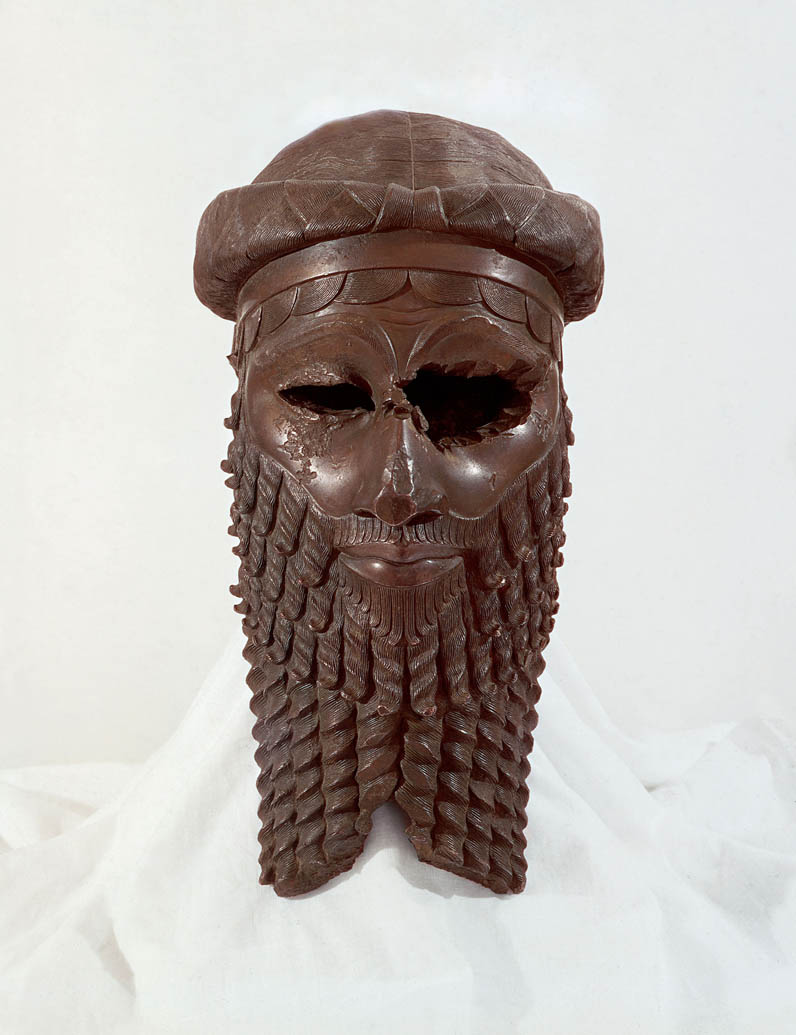
\includegraphics[height=120pt,keepaspectratio]{image1.png}\par
\vspace{4pt}
{\footnotesize Bronze head traditionally associated with Sargon of Akkad.\\Illustration supplied with the manuscript.}
\end{indented}
\clearpage
\FloatBarrier
\section{Introduction}\label{sec:2}

Over the past two decades, a particular kind of religious content has become common on the internet, especially on YouTube and more recently on short video platforms. This content presents itself as scientific. It usually involves a preacher or a content creator explaining that a verse from the Quran predicted something that science only discovered centuries later, or that an archaeological find has somehow confirmed a religious story. These videos often use the language of forensic science, medical imaging, and laboratory analysis. They are framed not as sermons but as evidence.

\begin{figure}[htbp]
\centering
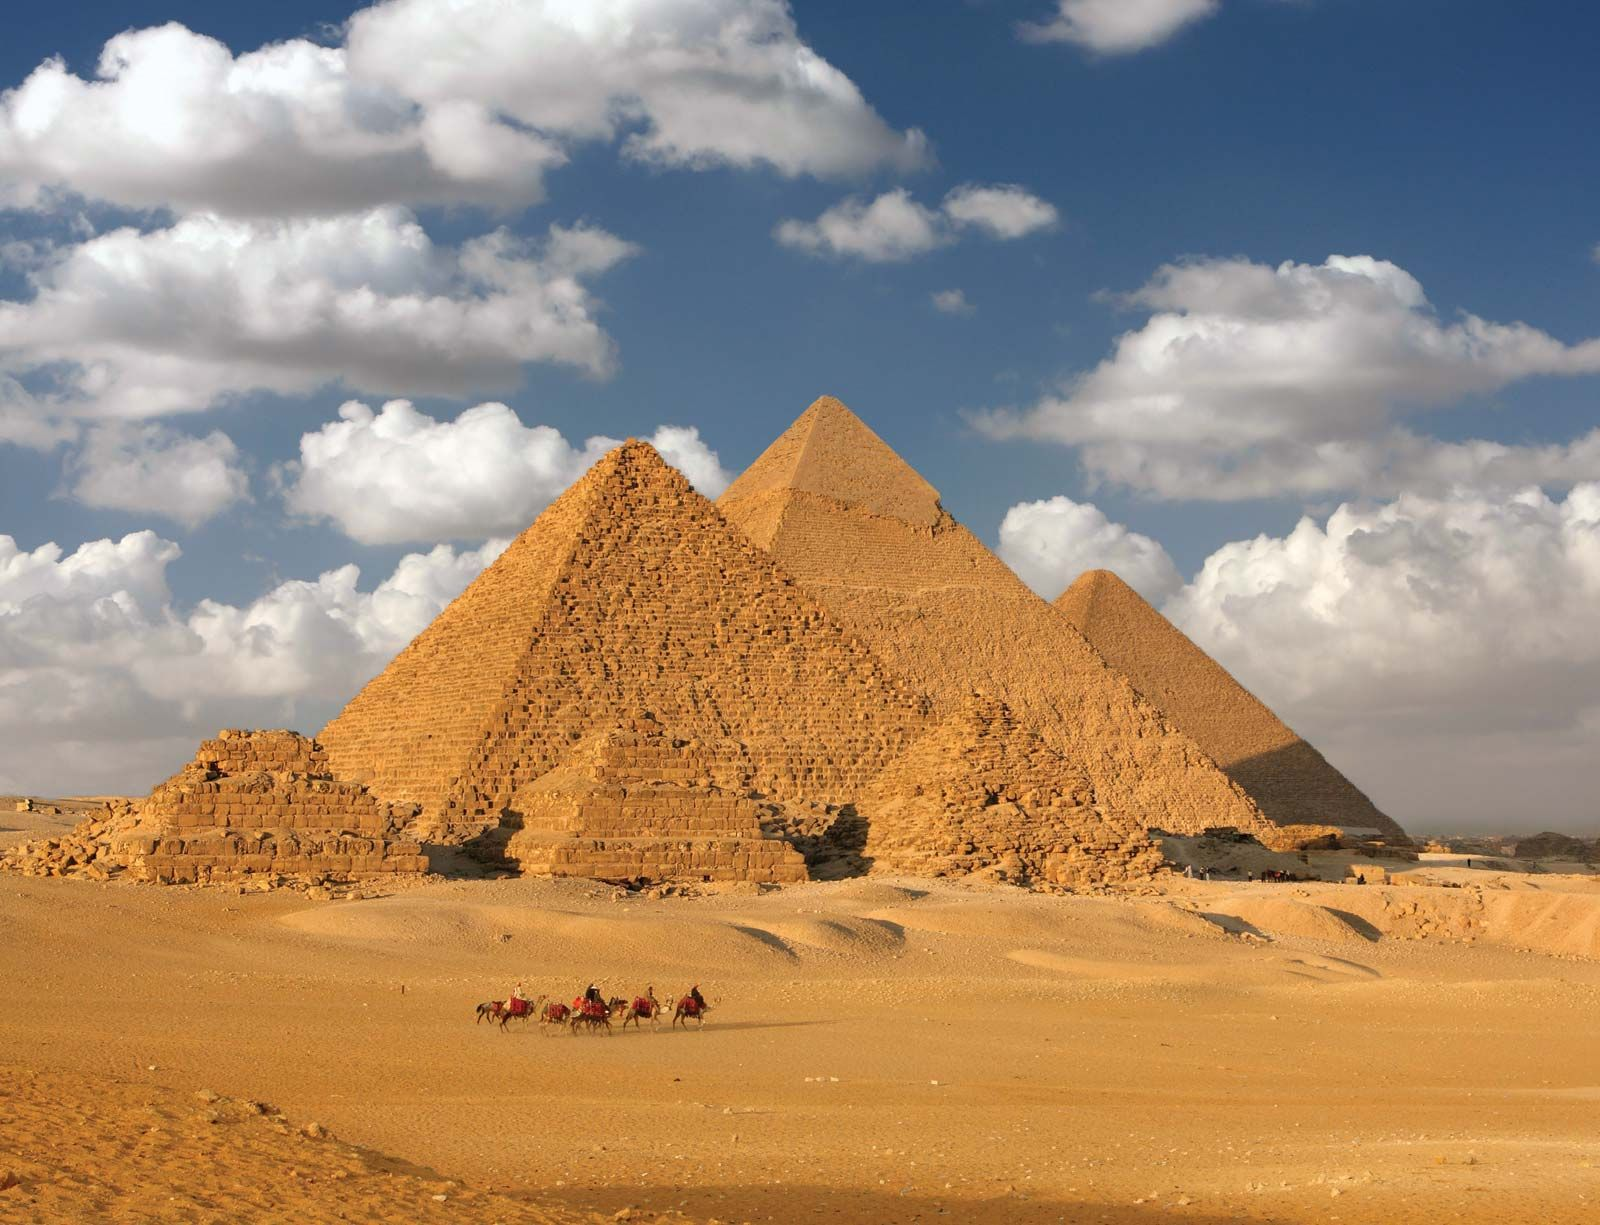
\includegraphics[width=.86\textwidth,height=.31\textheight,keepaspectratio]{image5.png}
\caption{Ancient Egypt's monumental civilization and mortuary culture formed the backdrop of later Exodus traditions.}\label{fig:1}
\end{figure}

One of the most widely circulated examples of this genre is the claim that the body of the Pharaoh who pursued Moses in the Exodus narrative was miraculously preserved by God, and that this body still exists today as physical proof of the Quranic account.

This type of argument did not begin on the internet. Its roots go back to a French physician named Maurice Bucaille, who published a book in 1976 titled The Bible, the Qur'an and Science . Bucaille argued that the Quran contained scientific knowledge that could not have been known at the time of its revelation, and that this was evidence of its divine origin. His work on the Pharaoh's body was one part of a larger project. Scholars who study this phenomenon often refer to it using the term Bucailism, named after him, to describe the broader practice of reading modern scientific findings back into religious texts as a form of proof. Bucaille was not a historian or an Egyptologist by training, and his conclusions were criticized fairly early on by specialists in those fields. Despite this, his arguments did not disappear. They were picked up, simplified, and repeated, first in print and later online, where they reached a much larger audience than Bucaille's original book ever could.

What makes the modern version of this claim worth studying is not just that it exists, but how it is presented. The Pharaoh's body claim is rarely framed today as a matter of faith or interpretation. It is framed as something closer to a courtroom exhibit. Content creators will show CT scan images, talk about salt residue on the skin, and describe the body in the language of forensic pathology. This creates the impression that the claim has already been tested and confirmed by science, when in most cases the actual scientific literature being referenced says something quite different, or is not being engaged with directly at all. The forensic packaging is part of what gives the claim its persuasive power. It borrows the authority of science without necessarily following the methods of science.

This paper is an attempt to take that claim seriously enough to actually test it, rather than simply accepting or rejecting it based on whether one already believes the underlying religious narrative. The approach taken here comes from historiography and comparative religion, two fields that are used to dealing with exactly this kind of problem, where a tradition makes a claim about the past and the question is what kind of evidence would actually support or undermine it. The goal is not to argue that the Exodus story is false, since that is a theological question outside the scope of this paper. The goal is narrower. It is to ask whether the specific historical and forensic claim, that a known mummy provides empirical proof of this particular verse, can survive ordinary historical scrutiny.

There are three problems with the claim that this paper will try to lay out carefully. The first is logical. The Quran's account refers only to ``Pharaoh,'' a title rather than a name. There is no dynasty given, no date, and no detail that would allow a historian to connect the text to one specific ruler out of the many pharaohs who held that title across Egyptian history. When apologists point to a mummy, usually Ramesses II or Merneptah, and treat its existence as confirmation of the verse, they are making a connection that the source text itself does not support. This is a version of a known logical error sometimes called affirming the consequent, where a possible explanation is treated as a confirmed one simply because it is consistent with the evidence, even when other explanations are equally or more consistent.

The second problem is statistical, or perhaps it is better to call it a problem of expectation. For a finding to count as evidence of something unusual, it has to be unlikely under normal circumstances. A preserved Pharaoh is not unlikely. Egyptian mummification was a highly developed, state level practice that was carried out routinely for roughly three thousand years. Finding a well preserved royal body in Egypt is closer to what one would expect by default than something that requires a special explanation. This point will come up again later in the paper, since it applies to both case studies discussed here.

The third problem is forensic, and this is where the paper spends the most time, since it is also where the apologetic claim is most specific and therefore most testable. Modern paleoradiology, particularly the CT scanning work carried out by researchers such as Sahar Saleem and Zahi Hawass on the royal mummies in Cairo, gives a detailed picture of how these bodies were prepared and what condition they were in at the time of death. This evidence does not point toward an unexplained natural preservation following a violent drowning. It points toward standard, highly invasive artificial mummification, the same process used on other Egyptian royalty who were not involved in any biblical or Quranic narrative at all. The salt found on these bodies, which apologists often describe as sea salt, is consistent with natron, the substance Egyptian embalmers used in the mummification process itself. The paper will go through this evidence in some detail in the first case study, including what is known about the age and physical condition of Ramesses II at the time of his death, since this evidence is fairly specific and worth examining closely rather than summarizing in passing.

The second case study in this paper turns to a different tradition within Islamic literature, the story of Namrud, often identified with the biblical Nimrod, who is said in some accounts to have died after a mosquito or gnat entered his brain as a form of divine punishment. This case was chosen partly because it follows a similar pattern to the Pharaoh claim, in that it presents a theological narrative as though it were also a historical record, and partly because it allows the paper to look at a case where the historical record is even thinner. Namrud does not appear by that name in any surviving Mesopotamian king list. The cities sometimes associated with him in later tradition were built by different rulers at different points in history, which creates real problems for treating Namrud as a single historical individual. Some scholars have suggested that Namrud may be a composite figure, drawing on the memory of earlier Mesopotamian kings such as Sargon of Akkad. This is presented in the paper as an interpretation rather than a settled fact, since the evidence for it is not as direct as the forensic evidence available for the Pharaoh case.

As a point of comparison, the paper also looks briefly at the death of Abu Jahl, a prominent opponent of Muhammad who was killed at the Battle of Badr in 624 CE. This case is included not because it is central to the paper's argument, but because it is useful as a kind of control. Abu Jahl's death is reported in early Islamic sources as an ordinary battlefield casualty, without supernatural elements attached to it. Looking at this case alongside the Pharaoh and Namrud narratives helps illustrate what a historically grounded claim tends to look like, as opposed to a legendary one, within the same broader literary and religious tradition.

It is worth being clear about what this paper is not trying to do. It is not trying to evaluate whether divine punishment, miracles, or supernatural preservation are possible in principle. Those are theological and philosophical questions, and they are not the kind of questions historical method is equipped to answer one way or the other. What this paper is trying to do is much narrower, and in some ways more mundane. It is asking whether two specific claims, both of which are presented online as historically and scientifically verified, actually hold up when measured against the kind of evidence historians normally require before accepting a historical claim. The same standard is applied to both cases, and the same standard would be applied to a similar claim made within any other religious tradition. This is meant as an exercise in historical method, not as an argument against any particular faith.

The paper proceeds as follows. The next section lays out the methodological framework used throughout, including the specific logical and evidentiary standards applied to each claim. This is followed by the first case study, on the Exodus Pharaoh, which is the longest section of the paper given the amount of forensic material available. The second case study addresses Namrud. A short comparative section then looks at Abu Jahl. The paper closes with a discussion of what these cases suggest about the difference between theological and historical claims, and a conclusion summarizing the main findings.

\FloatBarrier
\section{Methodological framework}\label{sec:3}

\subsection{Separating Theological Claims from Historical Claims}\label{subsec:3-1}

Before getting into specific tools of analysis, it helps to be clear about a distinction that runs through the entire paper. A theological claim is a claim that depends on faith, revelation, or religious authority for its truth. A historical claim is a claim about what actually happened in the past, and it depends on evidence that can in principle be checked by anyone, regardless of what they believe. These two types of claims often get mixed together in apologetic writing, sometimes on purpose and sometimes just because the writer has not thought carefully about the difference between them.

Take the Pharaoh case as an example. The claim that God preserved a body as a sign is a theological claim. It cannot be tested historically, because there is no method available to a historian for confirming or denying divine intervention. But the claim that a specific mummy, sitting in a museum in Cairo, shows physical evidence of having drowned and then being preserved through some process science cannot explain, is a historical claim. It is about a physical body, and physical bodies can be examined. This paper is only concerned with the second kind of claim. Where a claim cannot be tested by historical or forensic means, this paper says so directly and sets it aside rather than pretending to evaluate it.

This separation is not new or unique to this paper. It is a standard move in the historical study of religion, going back at least to nineteenth century biblical criticism, and it remains the basic working assumption of most historians who study religious texts today, regardless of which tradition they specialize in. Scholars working in this mode are not trying to settle whether a miracle happened. They are trying to figure out what the available evidence can and cannot support, which is a narrower and more answerable question.

It is also worth being honest about a limitation of this approach. Separating theological and historical claims works well on paper, but in practice the two are sometimes harder to pull apart, especially when a tradition's own internal logic treats a historical event as inseparable from its religious meaning. This paper tries to keep the separation as clean as possible, but it does not claim the separation is always perfectly tidy. Where a claim sits awkwardly between the two categories, this is noted rather than forced into one side or the other.

\subsection{Logical Standards: Two Fallacies}\label{subsec:3-2}

The first analytical tool used in this paper is fairly basic formal logic, specifically two related errors that show up repeatedly in apologetic arguments of this kind. Laying these out formally, rather than just describing them in passing, makes it easier to see exactly where the apologetic argument goes wrong.

The first is affirming the consequent. In its general form, this fallacy looks like this.

\begin{itemize}
\item Premise 1: If claim A is true, we would expect to observe B.
\item Premise 2: B has been observed.
\item Conclusion: Therefore A is true.
\end{itemize}

The problem with this structure is that finding B does not prove A, especially when B is also exactly what we would expect to observe under some entirely different explanation, call it C. In the Pharaoh case, the argument usually runs something like this.

Premise 1: If the Quranic account of a drowned and preserved Pharaoh is true, we would expect to find a preserved royal body. Premise 2: A preserved royal body has been found. Conclusion: Therefore the account is true.

The error is that a preserved royal body is exactly what we would also expect to find under explanation C, meaning that Egyptians mummified their kings as a matter of normal religious and political practice, regardless of whether any Exodus event occurred at all. Since the same observed evidence is consistent with both A and C, the evidence cannot be used to confirm A over C. It does not distinguish between them.

The second fallacy, related but slightly different, is the undistributed middle. This is a formal error in syllogistic reasoning where a conclusion is drawn from two premises sharing a middle term, but the middle term does not actually connect the premises the way the argument assumes. Applied loosely here, the issue is that the Quran's reference to Pharaoh functions as a general category, a title held by many different rulers across roughly three thousand years of Egyptian history, not a reference to one specific named individual. When an apologist identifies a particular mummy, often Ramesses II, and treats its discovery as confirmation of the verse, they are quietly supplying a piece of information the source text itself does not provide. The text says Pharaoh. It does not say which Pharaoh, in which dynasty, in which century. Treating a general title as though it picked out one verifiable individual creates the appearance of a logical connection that the actual text does not support.

This problem becomes more visible once you notice that apologists themselves do not agree on which mummy is meant. Some point to Ramesses II, others to Merneptah, and a few sources mention both without resolving the contradiction. If the identification were actually coming from the text, this disagreement would not exist, since the text would settle the matter. The fact that different writers land on different mummies suggests the identification is being supplied after the fact, based on which mummy seems to fit the story best, rather than being derived from any detail in the Quran itself.

A related issue, not a formal fallacy exactly but worth mentioning here, is what might be called the rhetorical use of scientific language as a stand in for actual scientific reasoning. When a claim is described using terms like forensic, CT scan, or empirical, it can sound more rigorous than it actually is, even when the underlying argument has not changed. This paper tries to be alert to this pattern throughout, since the difference between using a scientific term and applying a scientific method is exactly the gap this paper is interested in.

\subsection{The Baseline Expectation Rule}\label{subsec:3-3}

The third tool used in this paper is not a formal logical fallacy but more of a general principle borrowed from how historians and scientists usually evaluate claims of unusual or miraculous events. The basic idea is simple. For an observation to count as evidence of something extraordinary, the observation itself has to be unlikely or unexpected under ordinary circumstances. If the observation is exactly what we would expect anyway, for entirely mundane reasons, then it cannot serve as evidence for the extraordinary explanation, even if it is technically consistent with that explanation.

This idea is not original to this paper. A version of it goes back to the philosopher David Hume's discussion of miracles, and a more recent, looser version is sometimes summarized as the principle that extraordinary claims require extraordinary evidence. This paper does not need to take a position on Hume's broader argument about miracles to use a narrower version of the same idea here, which is that the strength of evidence has to be weighed against how likely that evidence was to appear anyway, for unrelated reasons.

This paper refers to this narrower version as the Baseline Expectation Rule. Applied to the Pharaoh case, the question is not simply whether a preserved royal mummy exists. It obviously does. The question is whether finding one is surprising. It is not. Ancient Egypt mummified its rulers as a matter of routine religious and state practice for roughly three millennia. Dozens of royal mummies have survived to the present day, the large majority of them with no connection to any biblical or Quranic narrative whatsoever. Finding a well preserved Pharaoh is close to the statistical default outcome of Egyptian royal burial practice, not an anomaly that requires a special explanation.

There is a cognitive dimension to this as well, which is worth flagging briefly even though this paper is not a psychology paper. Psychologists sometimes describe a pattern called base rate neglect, where people focus on a specific, vivid piece of evidence, such as a mummy looking dramatic on camera, while ignoring how common that type of evidence actually is in the broader population it comes from. The apologetic presentation of the Pharaoh's body leans heavily on this kind of framing. A single mummy is presented in isolation, without mentioning that dozens of similar mummies exist for rulers with no connection to the Exodus story at all. Once that wider context is included, the supposed anomaly mostly disappears.

The same rule will come up again in the Namrud case study, though in a different form, since the issue there is less about statistical likelihood and more about the complete absence of corroborating evidence for the figure in question in the first place.

\subsection{Hierarchy of Evidence}\label{subsec:3-4}

This paper draws on several different types of sources, and they are not all treated as equally reliable. Roughly in order of weight given to them:

Primary archaeological and forensic data carries the most weight in this paper. This includes CT scan results, paleoradiological reports, and direct physical examination of mummified remains, particularly the published work of researchers such as Sahar Saleem and Zahi Hawass. This kind of evidence has gone through peer review and is, at least in principle, open to being checked or challenged by other specialists working with the same imaging data.

Primary historical texts, including cuneiform king lists and early Islamic sources on figures such as Abu Jahl, are treated as important evidence but read with attention to genre, transmission, and purpose. A king list compiled for administrative or religious reasons is not the same kind of source as a modern excavation report, and the two are not held to identical standards of verification. Likewise, early Islamic historical and biographical sources, such as accounts of the Battle of Badr, come out of a tradition of historical writing with its own conventions, and this paper tries to read them on those terms rather than treating them as either fully equivalent to modern reporting or dismissing them outright.

Academic secondary literature, meaning peer-reviewed books and articles analyzing the primary evidence, is used throughout to interpret and contextualize the primary material. Disagreements among scholars in this literature are noted rather than smoothed over. Where this paper relies on a specific scholarly interpretation, such as the composite-figure theory for Namrud, it tries to be clear about whose interpretation it is and how widely it is accepted, rather than presenting it as uncontested consensus.

Apologetic and popular literature, including Bucaille's original work and its later online derivatives, is treated as the subject of analysis rather than as a source of evidence. In other words, this paper is not using Bucaille to find out what happened to Ramesses II. It is using Bucaille's claims as something to be tested against the primary forensic record. This distinction matters because apologetic literature is often written for a persuasive purpose rather than a descriptive one, which does not make it worthless as a source, but does mean it has to be read differently than a peer-reviewed excavation report.

\subsection{The Comparative Method}\label{subsec:3-5}

Since this paper sits partly within comparative religion, it is worth being explicit about what comparative actually means here. The method used in this paper is to apply the same evidentiary standard regardless of which religious tradition a claim comes from. The Pharaoh and Namrud cases both come from within an Islamic apologetic context, but the logical and forensic standards being applied to them are not specific to Islam. The same standards would apply to a similar claim made about, for example, a relic associated with a Christian saint, or a forensic claim made about a figure from Hindu or Buddhist tradition. This paper does not examine those other cases directly, since they are outside its scope, but the methodological symmetry is part of what keeps this paper from functioning as a one-sided critique of a single tradition.

This matters because critiques of religious miracle claims can sometimes end up applying a strict standard to one tradition while quietly assuming a more relaxed standard elsewhere, often without the author even noticing they are doing it. This paper tries to avoid that by stating its standard up front, in this section, before applying it to any specific case, so that the standard is fixed in advance rather than adjusted afterward to fit a preferred conclusion.

\subsection{Limits of Forensic Evidence on Ancient Remains}\label{subsec:3-6}

It is worth being upfront about what forensic and paleoradiological evidence can and cannot tell us, since the apologetic claims this paper examines sometimes lean on the authority of CT scanning without being precise about its actual limits.

CT imaging of mummified remains can show skeletal structure, evidence of disease or injury, the presence and placement of embalming material, and in some cases signs of how organs were removed during mummification. It can give a reasonably confident picture of a person's approximate age at death, general health, and certain types of trauma, particularly trauma to bone. What it generally cannot do is establish cause of death with the same certainty a modern autopsy could, since soft tissue has decayed or been removed, and chemical degradation over thousands of years limits what can be recovered. It also cannot, on its own, date when an injury occurred relative to death with perfect precision, though postmortem damage, such as breaks caused by later handling or robbery, can often be distinguished from injuries sustained while the person was alive, based on how bone responds differently to trauma before and after death.

This paper relies on the published interpretations of specialists working with this imaging, rather than trying to independently reinterpret CT data, since that level of technical judgment is outside the scope of a paper like this. Where the forensic literature itself expresses uncertainty about a particular finding, that uncertainty is carried over into this paper rather than resolved in favor of whichever conclusion is more convenient for the argument.

\subsection{Internal Critique Within Islamic Scholarship}\label{subsec:3-7}

One point that is easy to miss, and that this paper thinks is worth including, is that the criticism of Bucailism and the broader genre of scientific miracle claims, sometimes referred to in Arabic as i'jaz al ilmi, does not come only from outside observers such as Western Egyptologists or secular historians. A number of scholars working within Islamic studies and Quranic exegesis have also raised concerns about this genre, arguing that reading modern scientific findings back into the Quran represents a fairly recent interpretive innovation rather than a method grounded in classical tafsir tradition. Some of this criticism focuses on the same kind of problem discussed in section~\ref{subsec:3-2}, where a verse open to multiple readings gets matched retroactively to whatever the most recent scientific finding happens to be, which raises the question of what would have counted as a correct reading before that finding existed.

This paper does not attempt a full survey of this internal debate, since that would be a separate project on its own, but it is mentioned here because it changes the framing of this paper's argument somewhat. This is not simply a case of outside critics challenging a religious claim from outside the tradition. It is also a live methodological disagreement happening within Islamic scholarship itself, between those who see scientific miracle claims as a useful tool for da'wah, meaning religious outreach, and those who see it as a theologically risky departure from how the text has traditionally been read.

\subsection{Handling Uncertainty}\label{subsec:3-8}

Not every question in this paper has a clean answer, and the paper tries not to pretend otherwise. The Namrud case in particular involves more uncertainty than the Pharaoh case, since the forensic record available for an Egyptian mummy simply does not exist for a semi-legendary Mesopotamian king. Where the evidence supports a fairly confident conclusion, such as the mummification findings from CT imaging, this paper says so directly. Where the evidence only supports a plausible interpretation, such as the suggestion that Namrud may be a composite figure built from the memory of earlier rulers, this paper presents it as an interpretation, including noting which scholars hold this view and on what basis, rather than stating it as settled fact.

This paper also tries to use consistent language to signal its level of confidence, rather than letting word choice drift depending on which conclusion is being discussed. Phrases like the evidence shows or the data demonstrates are reserved for points with strong, peer-reviewed forensic or documentary support. Phrases like some scholars argue or this is consistent with are used for interpretive claims that are reasonable but not settled. The aim throughout is to match the strength of the conclusion to the strength of the evidence behind it, and to be upfront when that evidence runs out, rather than writing every section in the same confident tone regardless of how solid the underlying support actually is.

\FloatBarrier
\section{Case Study 1: The Exodus Pharaoh}\label{sec:4}

\subsection{The Textual Problem: An Anonymous Pharaoh}\label{subsec:4-1}

The starting point for this case study has to be the text itself, before getting into mummies or CT scans or anything forensic. The Quranic account of the Exodus, like the biblical account it parallels in many details, refers to the ruler who pursued Moses and his followers simply as Pharaoh. There is no personal name attached to him anywhere in the relevant verses. There is no dynasty mentioned, no regnal year, no reference to a particular city or monument that would let a historian narrow down which of Egypt's many pharaohs is meant. The verse most often cited in apologetic discussions, which describes God preserving the body of this Pharaoh as a sign for those who come after, does not specify whose body this is beyond the title itself.

This matters more than it might seem at first. Pharaoh was not a personal name. It was a title, used across roughly three thousand years of Egyptian history and applied to dozens of different rulers from different dynasties, different centuries, and in some cases different parts of Egypt entirely. Saying that a text refers to Pharaoh is a little like a modern text referring to the king or the president without saying which country or which year. It tells you something about the role being described, but it does not tell you who held that role at the time.

Historians who study the Exodus narrative, working from either the Quranic or biblical version, have never reached agreement on which Egyptian ruler the account might correspond to, assuming it corresponds to a specific historical event at all. Proposed candidates over the years have included Ramesses II, Merneptah, Thutmose III, Amenhotep II, and a few others, depending on which dating scheme a particular scholar favors. This disagreement has been going on for a long time and shows no sign of resolving, mostly because the textual evidence simply does not contain the kind of detail that would settle the question. Some scholars, working from a more minimalist position on the historicity of the Exodus, question whether a single identifiable Pharaoh and a single identifiable event lie behind the narrative at all, treating it instead as a national origin story shaped over a long period of oral and literary transmission. This paper does not take a position on that broader debate, since it goes well beyond the scope of a paper focused on the forensic evidence. The narrower point that matters here is simpler. Whatever the Exodus narrative is describing, the text does not name its Pharaoh, and any attempt to connect the verse to a specific mummy has to supply that missing identification from somewhere outside the text.

\subsection{Which Mummy? The Apologetic Disagreement Over Identity}\label{subsec:4-2}

\begin{figure}[htbp]
\centering
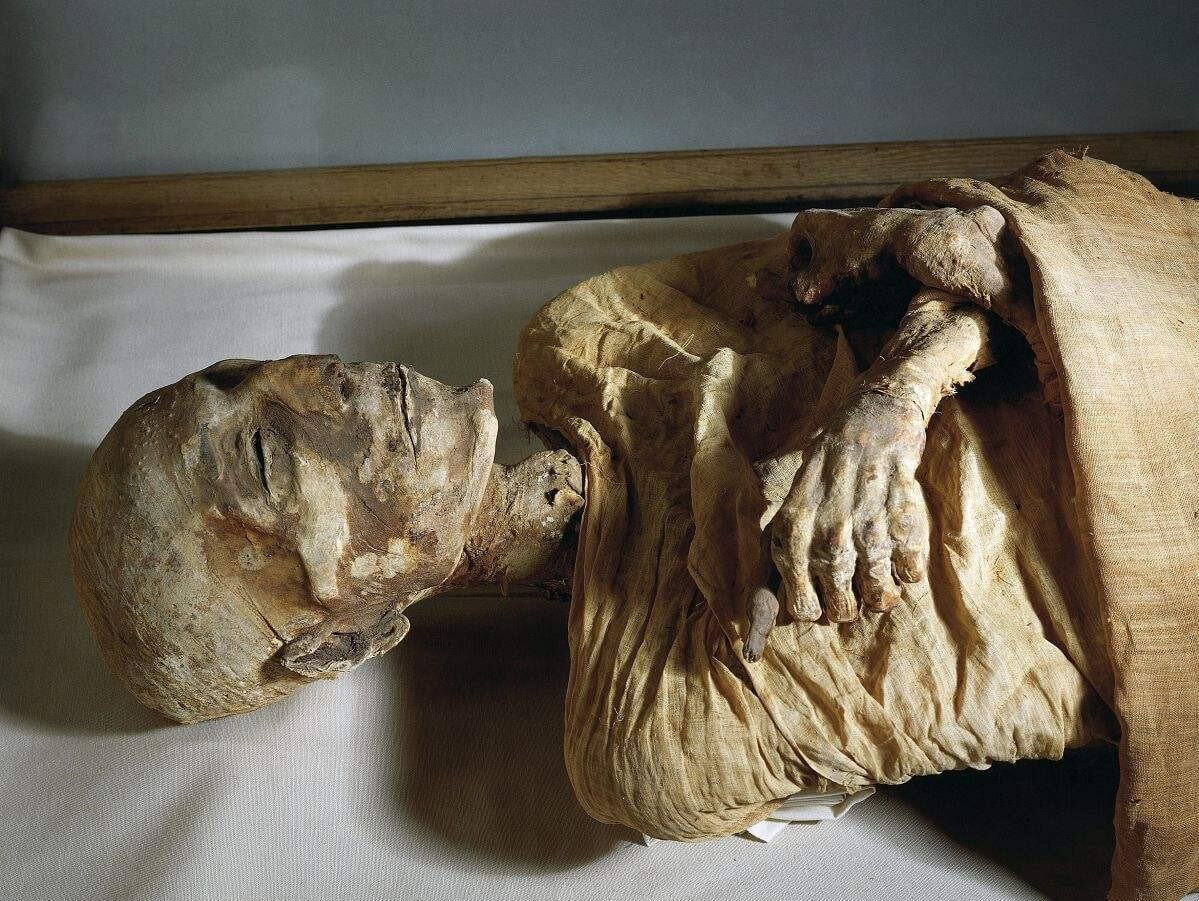
\includegraphics[width=.86\textwidth,height=.31\textheight,keepaspectratio]{image3.png}
\caption{Mummy of Merneptah, the Pharaoh emphasized in Bucaille's original investigation.}\label{fig:2}
\end{figure}

This is where the apologetic argument runs into its first real problem, and it is a problem that becomes obvious just by looking at how the claim has actually been made over the years rather than how it is described in summary.

If the claim were built on solid textual or historical grounds, one would expect apologists to agree on which mummy is being discussed. They do not. Maurice Bucaille, whose work is the origin point for most of the modern version of this claim, focused his attention on the mummy of Merneptah, since it was Merneptah's body that happened to be sent to Paris in the 1970s for conservation treatment, giving Bucaille direct access to it. Many popular presentations that followed Bucaille, however, shifted the focus to Ramesses II instead, partly because Ramesses II is the much more famous and visually striking mummy, and partly because Ramesses II fits more comfortably with the traditional, older popular assumption about who the Exodus Pharaoh was supposed to be, an assumption that predates Bucaille and goes back to older biblical scholarship and popular culture, including its long association in film and literature.

The result is a situation where two different mummies, belonging to two different rulers from two different points in the Nineteenth Dynasty, are both presented at different times and by different writers as the confirmed body of the Exodus Pharaoh. This is not a minor footnote. It points to the underlying weakness already discussed in the methodology section. If the identification were coming from the source text, this disagreement should not exist, since the text would settle the matter on its own. The fact that the identification shifts depending on which mummy happens to be available, photogenic, or convenient for a particular argument suggests that the connection is being made after the fact, fitted onto whichever body seems to suit the narrative best, rather than derived from anything the Quran or the underlying historical record actually specifies.

It is also worth being fair to the other side of this discussion. Some apologists have tried to resolve the inconsistency by arguing that more than one Pharaoh may be involved in the broader Exodus account, with one Pharaoh present during Moses's early life and a different one present during the Exodus itself, which is consistent with how the narrative is usually read. This is a reasonable attempt to deal with the inconsistency, and it shows that not every writer in this space is being careless. But even granting this point, it does not resolve the core issue, since the text still does not specify which ruler is meant by the pursuing Pharaoh whose body is said to be preserved. The disagreement over Merneptah versus Ramesses II is really a disagreement over which historical theory of the Exodus is correct, dressed up as though it were a settled forensic identification.

\subsection{Mummification as Routine Practice: Applying the Baseline Expectation Rule}\label{subsec:4-3}

\begin{figure}[htbp]
\centering
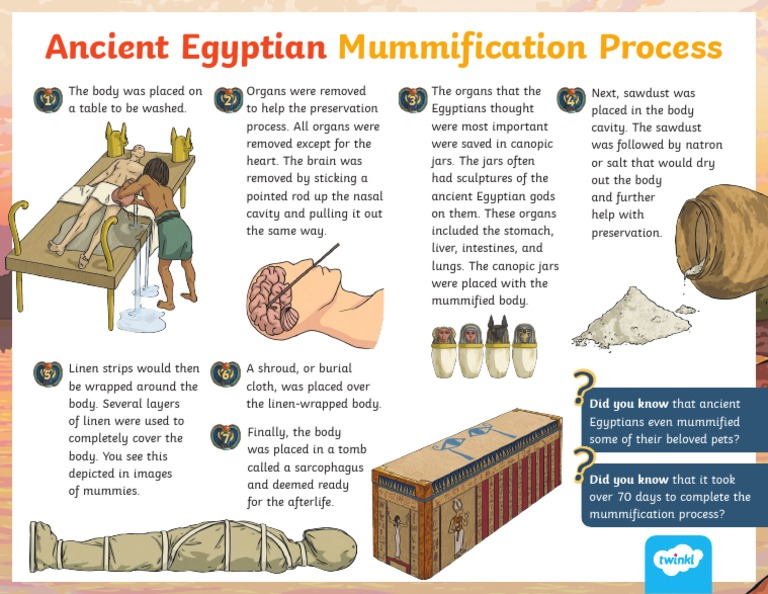
\includegraphics[width=.98\textwidth,height=.52\textheight,keepaspectratio]{image12.png}
\caption{Stages of Egyptian mummification, including organ removal, natron drying, and linen wrapping.}\label{fig:3}
\end{figure}

The methodology section introduced the Baseline Expectation Rule, the idea that an observation only counts as evidence for something extraordinary if that observation is itself unlikely under ordinary circumstances. This rule does a lot of work in this case study, so it is worth applying it carefully here rather than just gesturing at it.

Ancient Egyptian mummification was not a rare or occasional practice reserved for unusual circumstances. It was a standard part of Egyptian religious life for an extraordinarily long stretch of time, beginning in some basic form well before the Old Kingdom and continuing in increasingly elaborate forms through the New Kingdom and beyond, into the Greco-Roman period. Royal mummification in particular was highly developed by the time of the Nineteenth Dynasty, the period most often associated with Ramesses II and Merneptah. The process was carried out by trained embalmers as a matter of religious obligation, tied to beliefs about the afterlife and the preservation of the body as a vessel for the soul. This was not an improvised response to a particular crisis. It was an industrial scale, state supported practice that had been refined over many centuries by the time these two rulers died.

Given this, the discovery of a well preserved royal mummy from this period is not a surprising or anomalous event. It is close to the expected outcome. Dozens of royal and elite mummies from this same general period have survived to the present day, the great majority of them belonging to rulers and officials with no connection whatsoever to any Exodus narrative. Many of these mummies were deliberately moved by priests in later periods, particularly during the Twenty-first Dynasty, to protect them from tomb robbery, and were gathered into hidden caches such as the one found at Deir el-Bahari in the late nineteenth century. This cache alone contained dozens of royal mummies, including both Ramesses II and several other Nineteenth and Twentieth Dynasty rulers, none of whom are typically linked to the Exodus account.

The apologetic argument tends to present the existence of one preserved Pharaoh as though it were a striking exception to what we would normally expect to find. The broader archaeological record shows the opposite. Finding a preserved Pharaoh in Egypt is closer to a statistical certainty than an anomaly, given how routine and widespread the practice of royal mummification was. This does not, on its own, disprove anything about the Quranic narrative. What it does is remove one piece of evidence, the simple fact of preservation, from doing the work apologists want it to do, since that fact alone does not distinguish the Exodus account from the ordinary, well documented practice of Egyptian royal burial.

\subsection{Bucaille's Examination and the Origins of the Claim}\label{subsec:4-4}

\begin{figure}[htbp]
\centering
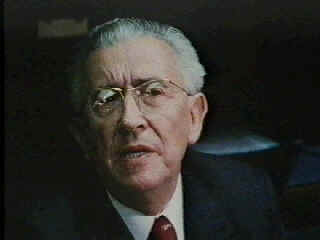
\includegraphics[width=140pt,height=105pt,keepaspectratio]{image6.png}
\caption{Maurice Bucaille, whose work popularized the preserved Pharaoh argument in modern apologetics.}\label{fig:4}
\end{figure}

It helps to look directly at where this specific claim comes from, since the modern, internet based version of the argument is almost always a simplified and often distorted descendant of one specific historical episode.

In 1975, the mummy of Merneptah was sent from Egypt to Paris as part of a conservation effort, since the mummy was showing signs of fungal deterioration and needed specialized treatment that was not available in Egypt at the time. Maurice Bucaille, a French physician with an interest in religious texts and a working relationship with the team handling the examination, was given access to the mummy during this period. Bucaille was not an Egyptologist by training and had no formal background in paleopathology or mummification studies. His interest in the mummy came from his broader project of trying to connect Quranic verses to scientific findings, a project that culminated in his 1976 book.

\begin{figure}[htbp]
\centering
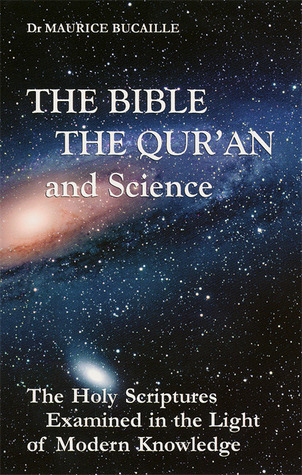
\includegraphics[width=.86\textwidth,height=.31\textheight,keepaspectratio]{image14.png}
\caption{Cover of Maurice Bucaille's The Bible, the Qur'an and Science. The edition depicted was not identified in the submitted material.}\label{fig:5}
\end{figure}

Bucaille reported finding salt deposits on the skin of the mummy, and he interpreted this as consistent with drowning, connecting it to the Quranic account of the Pharaoh's death and the promise that his body would be preserved. This interpretation became the foundation for the modern claim, repeated and simplified many times over in the decades since, often stripped of the qualifications and uncertainty present in Bucaille's own writing.

The reception of Bucaille's work among professional Egyptologists and historians of medicine was largely critical, and this criticism came fairly quickly after the book's publication. A central problem identified by specialists was that salt deposits on a mummified body are not, on their own, distinctive evidence of drowning. Salt residue is an expected feature of Egyptian mummification generally, since the embalming process itself relied heavily on a salt based substance to dry out the body. Bucaille's interpretation treated a routine feature of the embalming process as though it were a unique clue pointing to a specific cause of death, which is the same kind of error the methodology section described as affirming the consequent. Several Egyptologists at the time, and many since, have pointed out that Bucaille appeared to be unfamiliar with the basic chemistry and standard practice of Egyptian mummification, which undermined the central forensic claim his argument depended on.

It is fair to say that Bucaille's broader project, connecting modern science to Quranic verses, attracted both significant popular support and significant scholarly criticism, and that criticism came from multiple directions, including from within Islamic scholarship itself, where some scholars have raised concerns about the interpretive method involved, separate from the question of whether any particular scientific claim happens to be accurate.

\subsection{The Forensic Record: Saleem, Hawass, and the CT Evidence}\label{subsec:4-5}

The forensic picture available today is considerably more detailed than anything Bucaille had access to in the 1970s, mostly because of advances in computed tomography and the systematic CT scanning project carried out on the New Kingdom royal mummies by Egyptian and international researchers in the years since.

Sahar Saleem, a paleoradiologist, and Zahi Hawass, an archaeologist and former Egyptian Minister of Antiquities, have led much of this work, publishing detailed CT based studies of multiple royal mummies including Ramesses II and other Nineteenth and Twentieth Dynasty rulers. This research is published in peer-reviewed academic venues and represents a far more systematic and technically detailed examination than anything available to Bucaille.

The CT findings on these mummies are broadly consistent with standard, highly invasive Egyptian embalming practice rather than any unexplained or unusual mode of preservation. The scans show clear evidence of evisceration, meaning the surgical removal of internal organs, a routine step in high status Egyptian mummification intended to slow decomposition. They show evidence consistent with the standard method of brain removal through the nasal cavity, another well documented step in the embalming process for elite burials during this period. They show packing material inside the body cavity, linen wrapping applied in the expected, methodical way, and skeletal and dental features consistent with what is known about the embalming and wrapping conventions of the period.

None of this is presented in the CT literature as evidence of an unexplained, miraculous, or scientifically anomalous mode of preservation. It is presented, plainly, as confirmation that these bodies went through the same artificial, human directed mummification process used on Egyptian royalty generally, with no distinguishing features that would set them apart from other mummies of the same period who have no connection to any Exodus narrative. This is a meaningful point. If the body in question had been preserved through some process science could not explain, the CT evidence would presumably show something unusual, some deviation from the standard mummification pattern seen in other royal mummies from the same dynasty. Instead, what the scans show is closely consistent with ordinary practice.

The two CT illustrations reproduced here are of Amenhotep I. They are comparative material, not scans of Ramesses II. Saleem and Hawass (2021) found that Amenhotep I's brain remained in place and did not establish a cause of death from CT. This example shows why findings about one mummy cannot simply be transferred to another. The present paper reports no original CT examination or chemical analysis.

\subsection{Natron, Not Seawater}\label{subsec:4-6}

\begin{figure}[htbp]
\centering
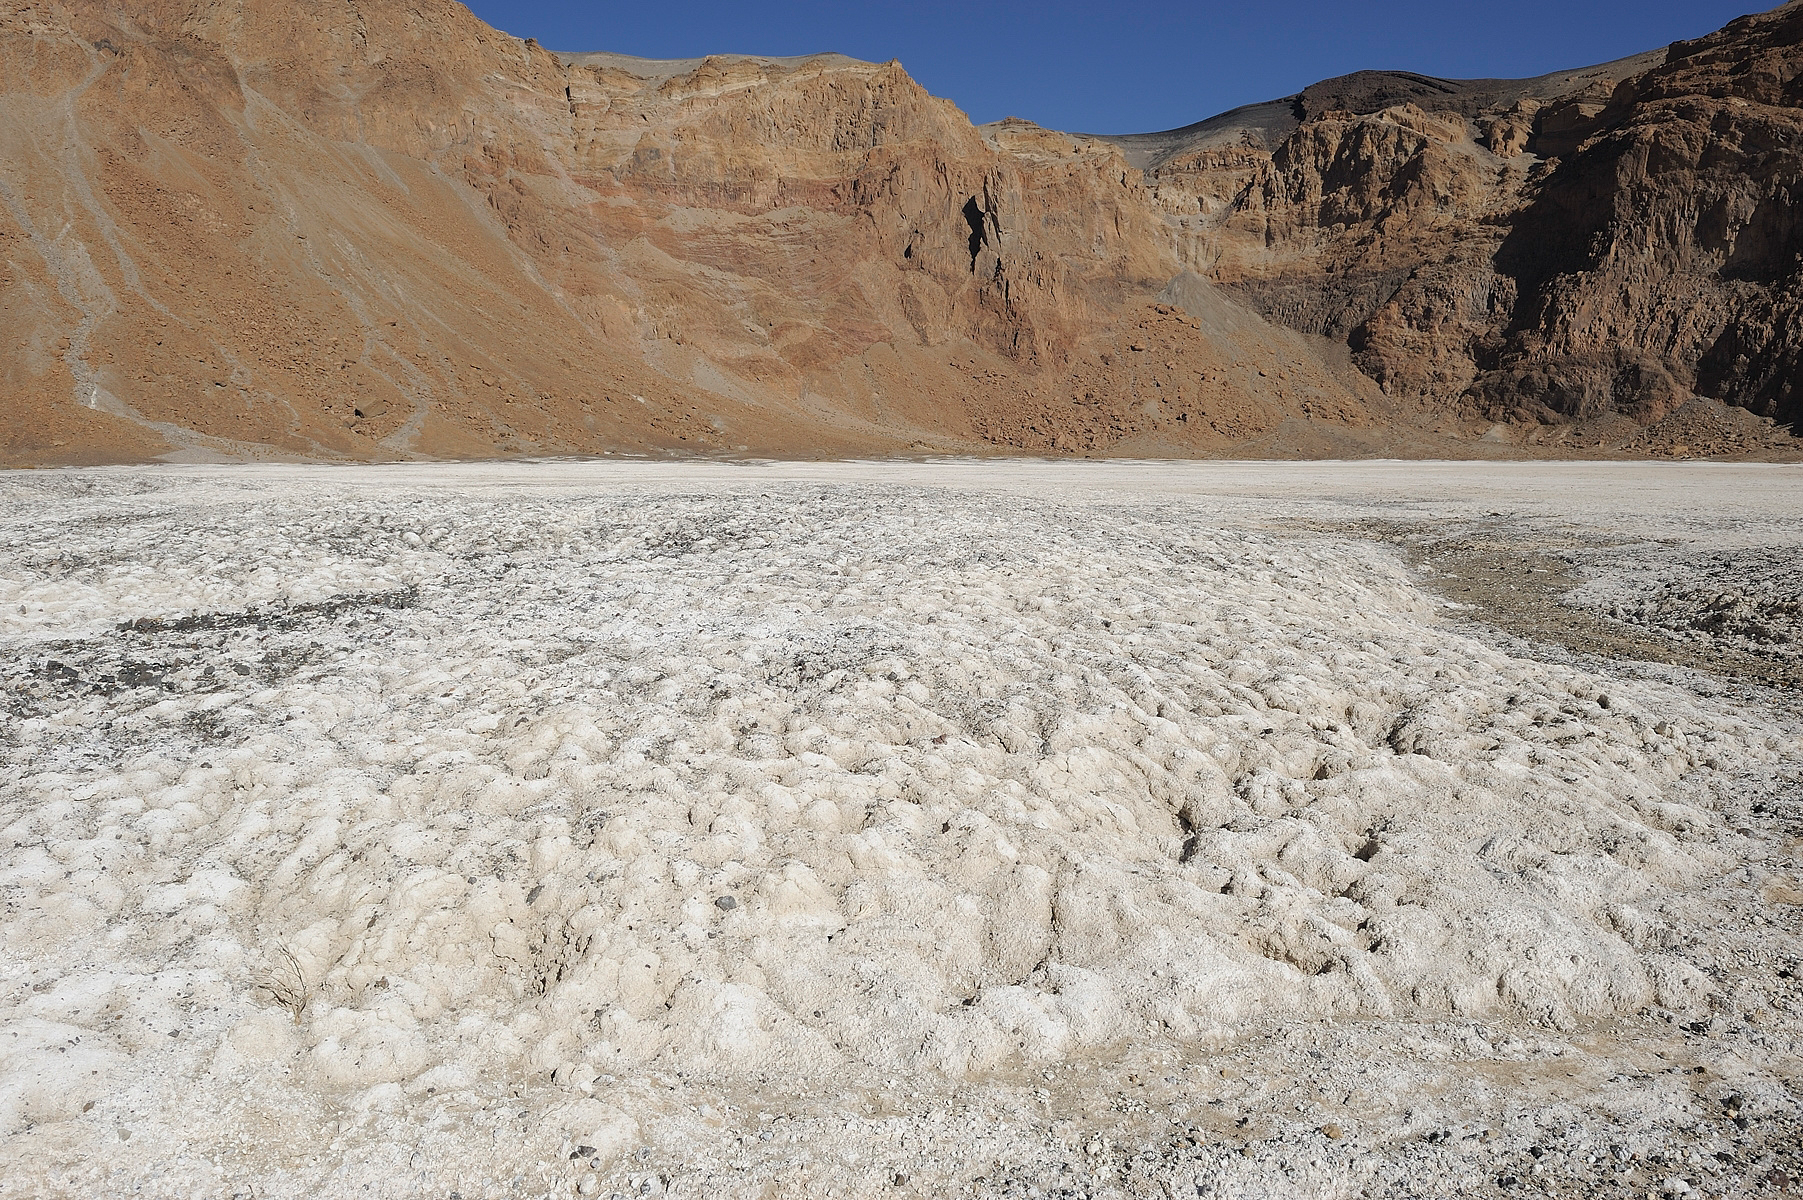
\includegraphics[width=.86\textwidth,height=.31\textheight,keepaspectratio]{image13.png}
\caption{Evaporite deposits, retained as a general illustration. The photograph alone does not identify the minerals or establish the source of residues on a mummy.}\label{fig:6}
\end{figure}

The salt question deserves its own closer look, since it sits at the center of the original Bucaille claim and remains central to how the argument is presented online today.

Natron is a naturally occurring mineral salt mixture, made up primarily of sodium carbonate and sodium bicarbonate along with smaller amounts of sodium chloride and sodium sulfate. It occurs naturally in certain dry lake beds in Egypt, most famously in the Wadi Natrun region, which gives the substance its name. Egyptian embalmers used natron as the primary desiccating agent in mummification, packing it around and sometimes inside the body to draw out moisture and prevent decay. Ancient sources, including the Greek historian Herodotus, describe this process, including a drying period of roughly forty days, though the precise duration and method varied somewhat across periods and social classes.

The presence of salt residue on a mummified body, then, is exactly what one would expect to find on any properly embalmed Egyptian mummy, royal or otherwise, regardless of how that person died. It is not a special or unusual feature limited to bodies that drowned. Bucaille's original interpretation treated salt on the skin as though it pointed specifically toward seawater and therefore toward drowning, but this does not hold up well against what is actually known about the embalming process. Natron residue and seawater residue are chemically distinguishable, since natron's composition, dominated by carbonate and bicarbonate compounds, differs from the composition of seawater, which is dominated by sodium chloride. Later analysis and broader knowledge of mummification chemistry have generally supported the natron explanation over the seawater explanation, since natron use in mummification is independently well documented through both textual and archaeological evidence, while the seawater claim depends entirely on accepting the Exodus narrative as historical fact first and then reading the salt evidence backward to fit it.

This is, again, the same logical structure discussed earlier. A piece of evidence, salt residue, that is fully explained by an ordinary, well attested cause, embalming practice, is instead treated as confirmation of an extraordinary cause, drowning followed by miraculous preservation, without good reason to prefer the extraordinary explanation over the ordinary one.

\subsection{Ramesses II: Age, Health, and Cause of Death}\label{subsec:4-7}

\begin{figure}[htbp]
\centering
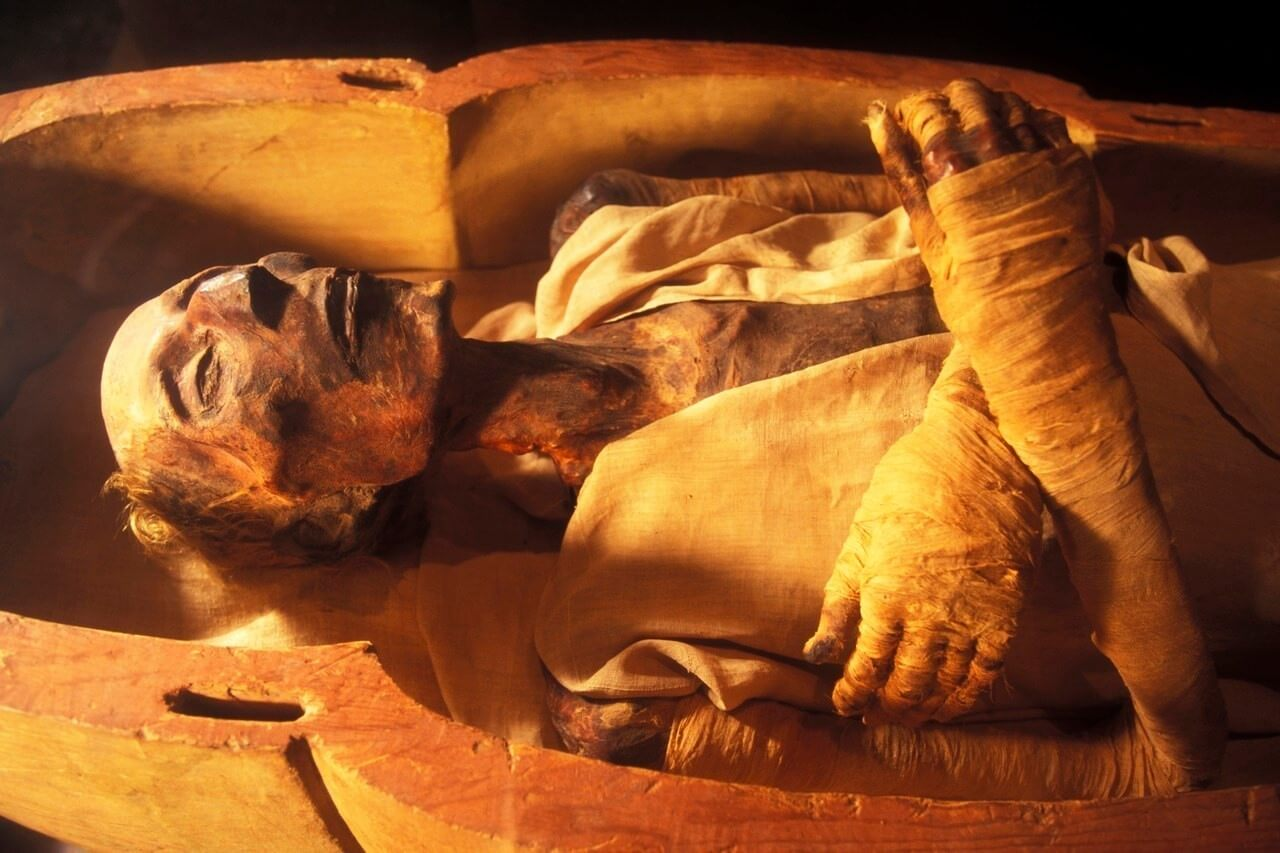
\includegraphics[width=.86\textwidth,height=.31\textheight,keepaspectratio]{image10.jpg}
\caption{Ramesses II, one of the most frequently proposed candidates for the Exodus Pharaoh.}\label{fig:7}
\end{figure}

\begin{figure}[htbp]
\centering
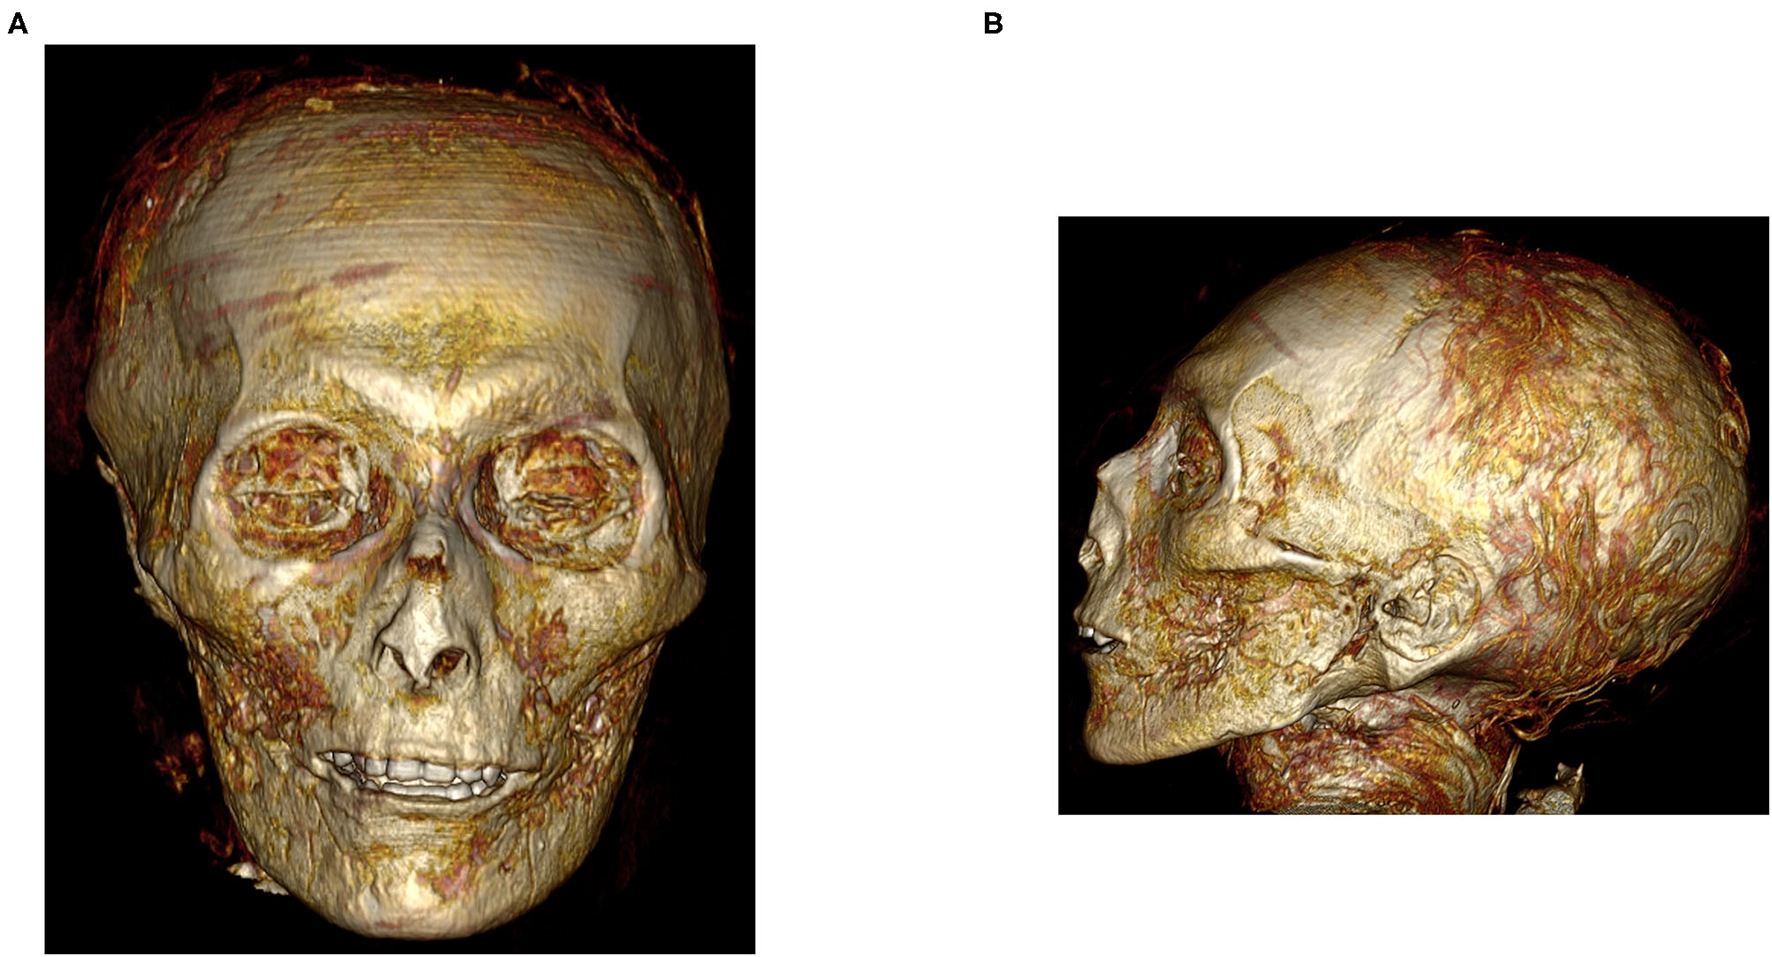
\includegraphics[width=.86\textwidth,height=.31\textheight,keepaspectratio]{amenhotep-figure3.png}
\caption{CT rendering of the face of Amenhotep I, used here as a comparative example of digital unwrapping, not as evidence about Ramesses II. Saleem and Hawass (2021), figure 3, CC BY.}\label{fig:8}
\end{figure}

\begin{figure}[htbp]
\centering
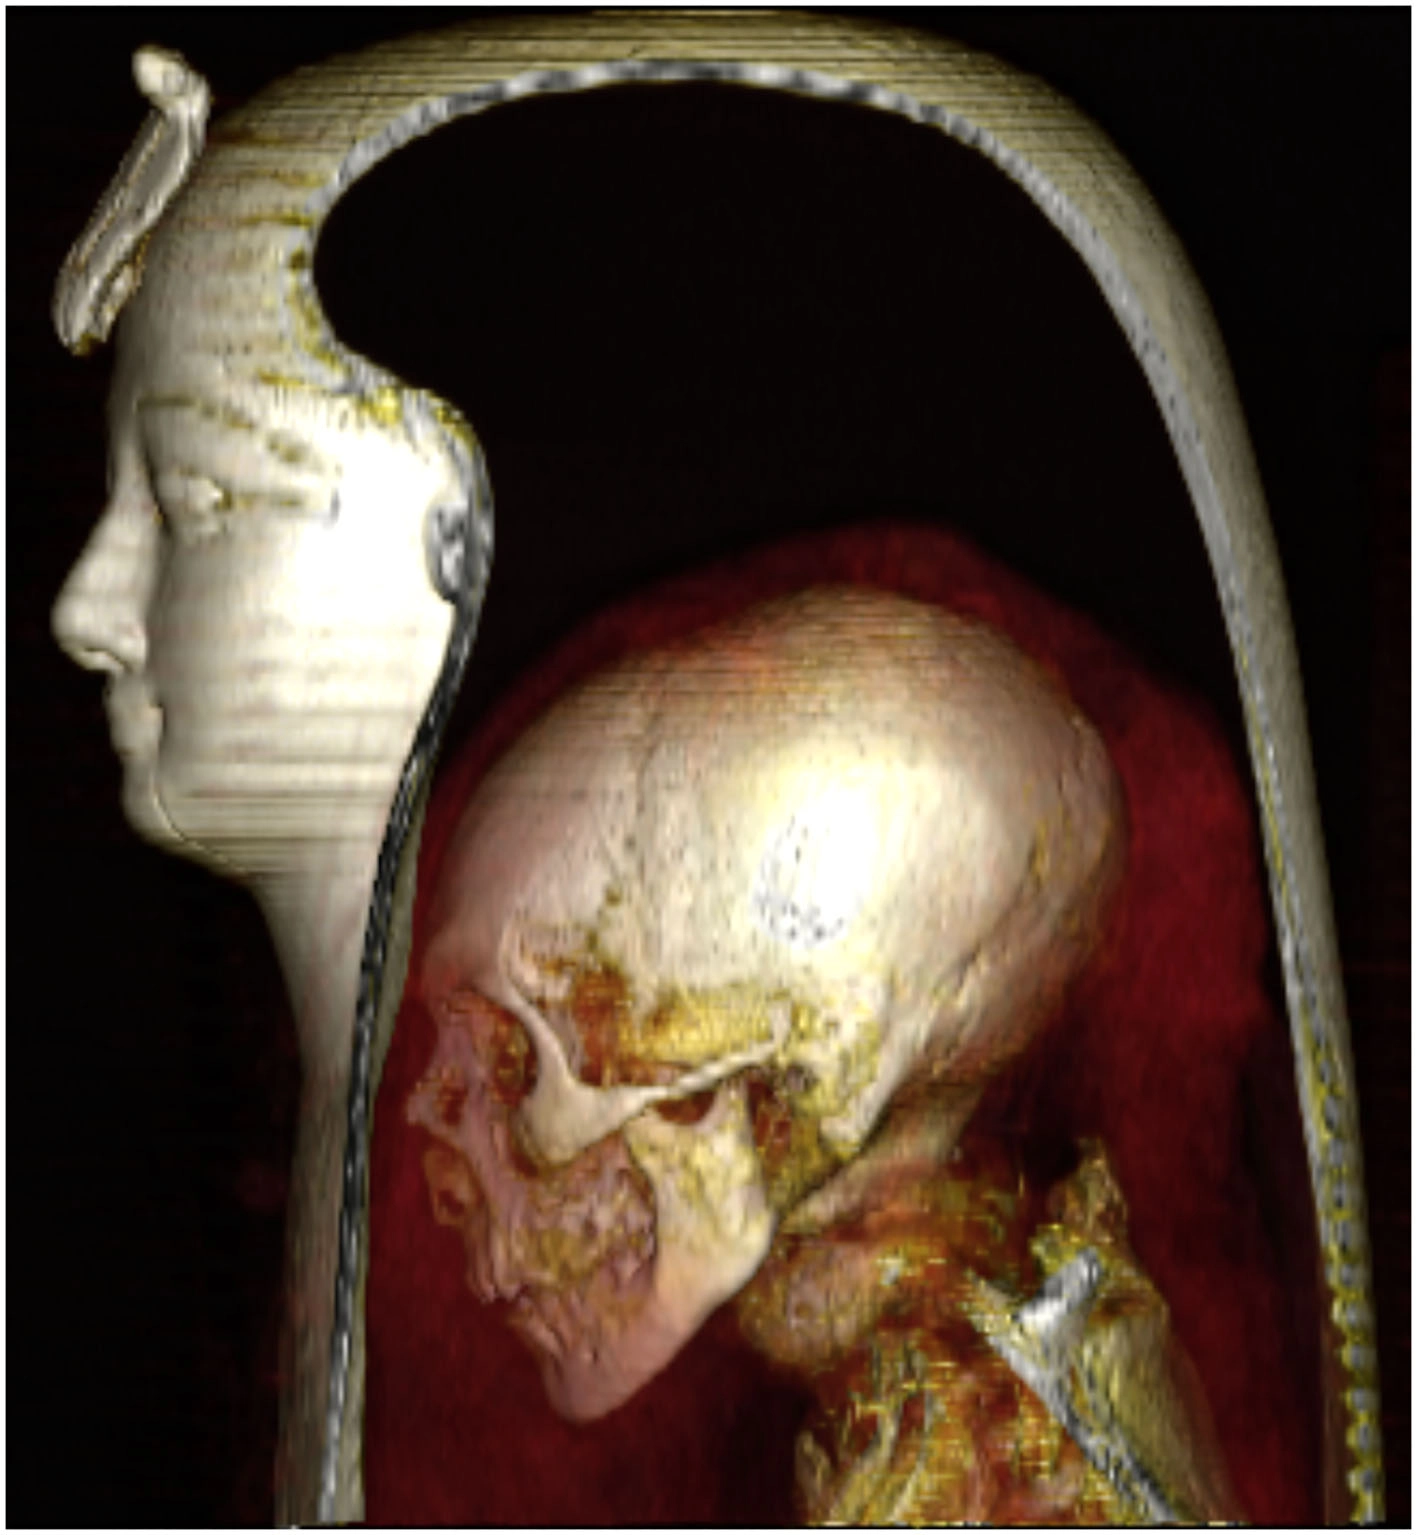
\includegraphics[width=.86\textwidth,height=.31\textheight,keepaspectratio]{amenhotep-figure2.png}
\caption{CT rendering of the head, mask, and wrapping of Amenhotep I. This is a different individual from Ramesses II. Saleem and Hawass (2021), figure 2, CC BY.}\label{fig:9}
\end{figure}

Since Ramesses II is the mummy most often invoked in popular versions of this claim, it is worth looking specifically at what the forensic record says about him as an individual, rather than treating the case only in general terms.

Based on skeletal and dental analysis, most researchers place Ramesses II's age at death somewhere around ninety, an unusually long life by the standards of the ancient world and consistent with the historical record of his reign, which lasted around sixty-six years, one of the longest reigns in Egyptian history. The CT and earlier X-ray studies of his remains show significant degenerative changes consistent with advanced age, including severe arthritis affecting his joints and spine, along with evidence of dental disease, including abscesses and significant wear, conditions that would have been a source of real discomfort in his later years. There is also evidence in the literature of vascular calcification consistent with atherosclerosis, a condition associated with aging.

These findings establish advanced age and degenerative disease. They do not, by themselves, establish the immediate cause of death. Old age and arthritis cannot exclude drowning. The relevant conclusion is narrower: the evidence discussed here does not provide a secure, independent diagnosis of drowning, and identification of the mummy as the Pharaoh of the narrative remains unestablished.

It is worth being careful here about what this paper is and is not claiming. The forensic record cannot, on its own, prove or disprove whether Ramesses II is or is not the figure described in the Exodus narrative, since that identification was never secure in the first place, for the textual reasons discussed in section~\ref{subsec:4-1}. What the forensic record can do is undercut the specific physical narrative often attached to this mummy in popular apologetic presentations, the idea of a Pharaoh whose body shows direct physical evidence of death by drowning. The observations discussed here do not supply that diagnosis.

\subsection{The Fractures: Tomb Robbery, Not Drowning}\label{subsec:4-8}

\begin{figure}[htbp]
\centering
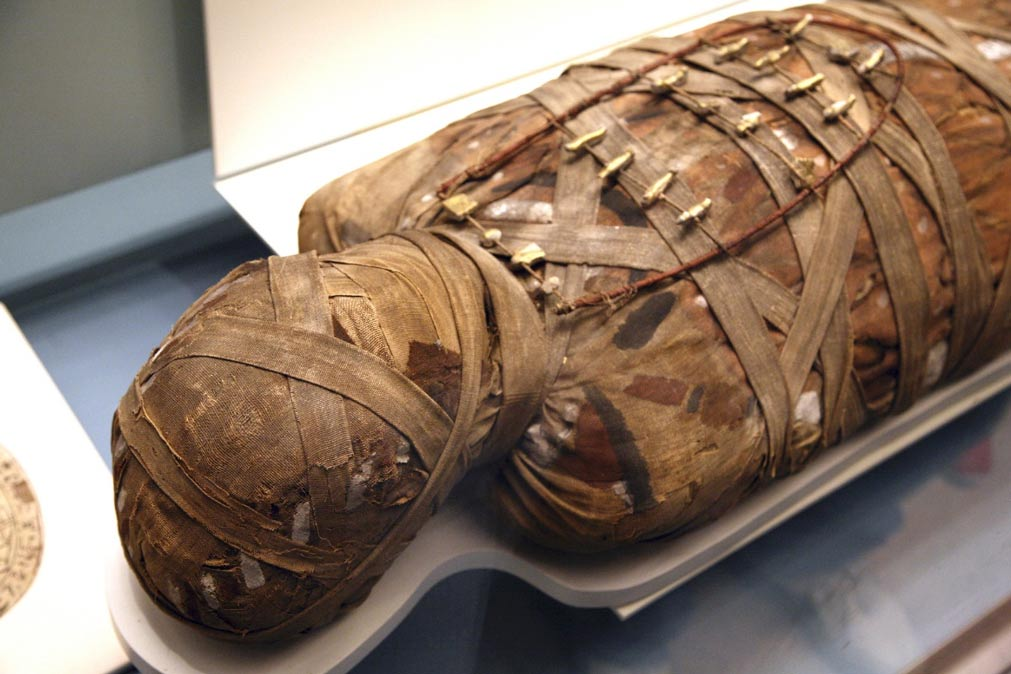
\includegraphics[width=.86\textwidth,height=.31\textheight,keepaspectratio]{image9.png}
\caption{Linen wrapping and resin hardening characteristic of Egyptian mummification.}\label{fig:10}
\end{figure}

Some popular presentations of this claim point to skeletal fractures found on certain royal mummies, including Ramesses II, as further physical evidence of violent death, sometimes framed as consistent with a chaotic or forceful event such as drowning. The forensic literature offers a different and fairly well supported explanation for this damage.

Many of the royal mummies recovered from caches such as Deir el-Bahari and the tomb of Amenhotep II show evidence of damage caused after death, often centuries after death, by ancient tomb robbers searching for valuable amulets and jewelry that were commonly wrapped within the linen bandages of high status burials. This robbery activity is itself well documented historically, and it is part of the reason the royal mummies were moved from their original tombs to hidden caches in the first place, an effort by priests during a period of political instability to protect the bodies from further desecration. The process of searching through hardened, resin soaked linen wrappings for hidden valuables could be rough, and it sometimes resulted in damage to the body underneath, including fractures to bones that had become brittle over time.

Forensic researchers working with CT imaging are generally able to distinguish, at least to a reasonable degree, between trauma that occurred while a person was alive, which tends to show particular healing or bleeding patterns, and damage that occurred after death, particularly damage that occurred long after death once the body and its wrappings had already dried and hardened. Where this kind of postmortem damage has been documented on royal mummies, the explanation favored by researchers working directly with the physical evidence tends to point toward later disturbance by robbers rather than violence at the time of death. This is presented in the literature with appropriate caution, since distinguishing ancient postmortem damage with full certainty is not always straightforward, but the explanation grounded in documented tomb robbery activity fits the broader historical and archaeological context far better than an undocumented and physically unsupported drowning event.

\subsection{The Philosophical Problem: A Miracle That Required Embalmers}\label{subsec:4-9}

Setting the forensic detail aside for a moment, there is a more basic problem with how this claim is constructed, one that does not require any CT scan to notice.

The Quranic account, as discussed earlier, describes the preservation of the Pharaoh's body as a sign, something framed as an act outside the ordinary course of nature. But the body actually being pointed to in the apologetic argument is not a body preserved through some unexplained or extraordinary process. It is a body that went through the full, standard, labor intensive Egyptian mummification process, the same process applied to thousands of other Egyptians of sufficient rank across three thousand years of history. This process required teams of trained human embalmers. It required cutting open the abdomen to remove internal organs. It required inserting a hooked instrument through the nasal cavity to extract and discard the brain, since Egyptian embalmers generally regarded the brain as unimportant for the afterlife. It required packing the body cavity and surrounding the body with natron over a period of weeks to draw out moisture, followed by careful wrapping in resin treated linen.

If the explanation being offered is that this body was supernaturally preserved as a sign defying the ordinary processes of decay, it sits awkwardly next to the fact that the body's preservation depended entirely on an elaborate, well understood, thoroughly human technical process, one that left behind exactly the kind of physical evidence, surgical incisions, missing organs, embalming residue, that one would expect from artificial preservation rather than anything outside the ordinary course of nature. A body preserved by direct supernatural intervention, defying the normal rules of decomposition, would not obviously need its organs removed by hand and its brain extracted through the nose first.

This paper does not present this point as a logical disproof of the underlying theological claim, since a believer could reasonably respond that the preservation was achieved precisely through the human embalming process, with the miracle being one of circumstance or timing rather than a violation of the embalming process itself. That is a coherent theological position, and this paper is not in a position to rule it out. But it is worth pointing out clearly that this version of the claim is a different, more modest claim than the one usually presented in popular apologetic content, where the language used tends to suggest a body preserved in a way science cannot explain. The actual forensic picture is the opposite of unexplained. It is, in fact, one of the more thoroughly documented and well understood preservation processes in the ancient world.

\subsection{Summary of Findings}\label{subsec:4-10}

Pulling these threads together, the case against treating a specific mummy as empirical proof of the Quranic Pharaoh narrative rests on several separate but related points, each of which holds up independently of the others.

The source text does not name a specific Pharaoh, which means any identification of a particular mummy has to be supplied from outside the text, and apologists themselves have not agreed on which mummy this should be. Egyptian royal mummification was a routine, widespread practice across three thousand years, which means a preserved Pharaoh is an expected possible result of royal burial practice rather than, on that fact alone, an anomaly requiring a special explanation. The original claim traces back to Maurice Bucaille's 1975 examination of Merneptah's mummy, an examination criticized by Egyptologists for misunderstanding standard embalming chemistry. Modern CT based forensic work by researchers such as Sahar Saleem and Zahi Hawass shows mummification consistent with standard practice rather than any unexplained mode of preservation. The salt residue central to the original claim is well explained by natron, the documented embalming agent, rather than seawater. Ramesses II shows advanced age and degenerative disease; these observations neither establish his immediate cause of death nor exclude drowning. Skeletal damage on some royal mummies is better explained by documented ancient tomb robbery than by any drowning event. And the underlying logic of the claim sits in some tension with itself, since a body preserved through elaborate, well documented human embalming technique is a strange candidate for evidence of preservation outside the ordinary course of nature.

None of this, on its own, settles the theological question of whether the Exodus account is true. That question, as the methodology section explained, is not one historical or forensic method is equipped to answer. What this case study has tried to show is something narrower and more specific, that the particular empirical claim built around a named mummy does not hold up well against the available textual, archaeological, and forensic evidence, and that the persuasive force of the claim depends heavily on details, especially around salt and physical condition, that do not match what the primary research literature actually documents.

\FloatBarrier
\section{Case Study 2 : Namrud}\label{sec:5}

\subsection{The Narrative and Its Textual Layers}\label{subsec:5-1}

Before looking at the historical record, it helps to separate out where the Namrud story actually comes from, since this gets blurred in most popular presentations of it.

The Quran itself does not use the name Namrud. The relevant passage, in Surah Al-Baqarah, describes a dispute between Abraham and an unnamed king who claimed power over life and death, a king who grew arrogant and rejected Abraham's argument about God. Classical commentators identified this king as Namrud, drawing on a name and a set of associated traditions that were already circulating in Jewish and Near Eastern literature before Islam. The detailed story most people are familiar with today, the building of a tower, the attempt to reach the heavens, the fire Abraham was thrown into and survived, and especially the death by a gnat or mosquito entering the brain, comes from a different layer of material. It comes from tafsir, meaning Quranic commentary, and from a genre of literature called qisas al-anbiya, or tales of the prophets, which collected and elaborated on stories about earlier prophets using material drawn partly from Jewish tradition, partly from older Near Eastern legend, and partly from later storytelling embellishment.

This kind of material is sometimes referred to within Islamic scholarship as Israiliyyat, a term used for narrative traditions absorbed into Islamic literature from Jewish and other outside sources. It is worth being clear that this is not a term invented by outside critics to dismiss the tradition. Classical Muslim scholars themselves, including well known exegetes, treated Israiliyyat material with caution, distinguishing it from material with a clear chain of transmission back to the Quran or to reliable hadith. The mosquito death story falls into this more cautious category. It is a long standing and widely repeated part of the tradition, but it does not carry the same evidentiary status as the Quranic text itself, and this distinction matters for a paper trying to evaluate the story's historical claims rather than its theological standing.

\subsection{Absence from Native Mesopotamian King Lists}\label{subsec:5-2}

\begin{figure}[htbp]
\centering
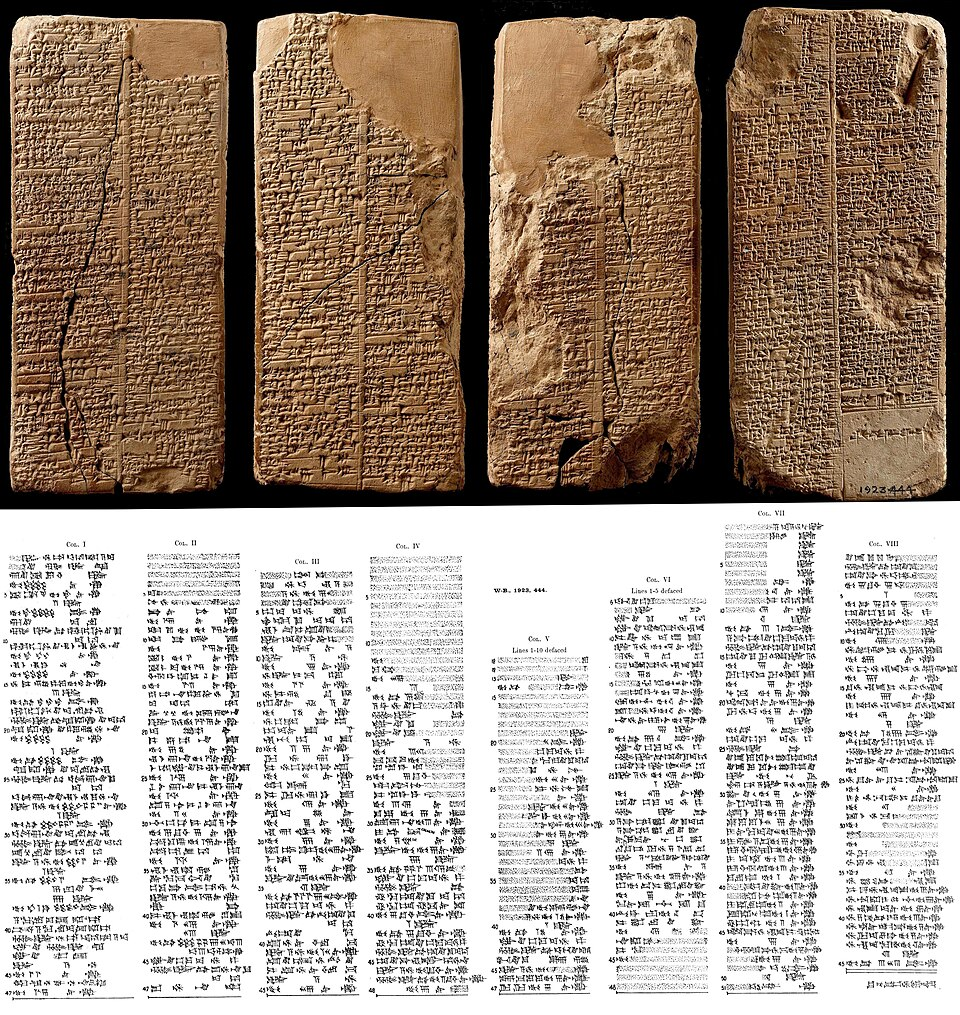
\includegraphics[width=.86\textwidth,height=.31\textheight,keepaspectratio]{image11.png}
\caption{The Sumerian King List, one of the principal sources used to reconstruct Mesopotamian rulership.}\label{fig:11}
\end{figure}

The historical record for ancient Mesopotamia is, in some ways, unusually good compared to other parts of the ancient world, because Mesopotamian scribes kept detailed king lists recording rulers, the length of their reigns, and the cities they governed. The Sumerian King List, along with later Assyrian and Babylonian king lists, gives historians a reasonably continuous, if not always perfectly reliable, record of rulership across the region stretching back well over four thousand years.

No version of these lists contains a ruler named Namrud, or any clear variant of that name, in connection with the kind of figure described in later legend, a singular, world dominating tyrant king associated with Babel, Erech, Akkad, and Calneh all at once. This absence is not simply a gap caused by missing records, since the surviving king lists are reasonably extensive for the periods in question. It is worth being careful here, since absence of evidence is not automatically proof that no such person existed under a different name, and ancient king lists were themselves sometimes compiled for political or religious purposes that shaped which rulers were included and how their reigns were described. But the consistent absence across multiple independent native sources does mean that Namrud, as a specific individual with that name and that specific scope of rule, has no direct anchor in the primary Mesopotamian historical record. Anyone treating Namrud as a straightforwardly historical figure has to explain this absence, and most serious treatments of the question do attempt some kind of explanation, usually along the lines discussed in section~\ref{subsec:5-4} below.

\subsection{The City-Founding Anachronism}\label{subsec:5-3}

\begin{figure}[htbp]
\centering
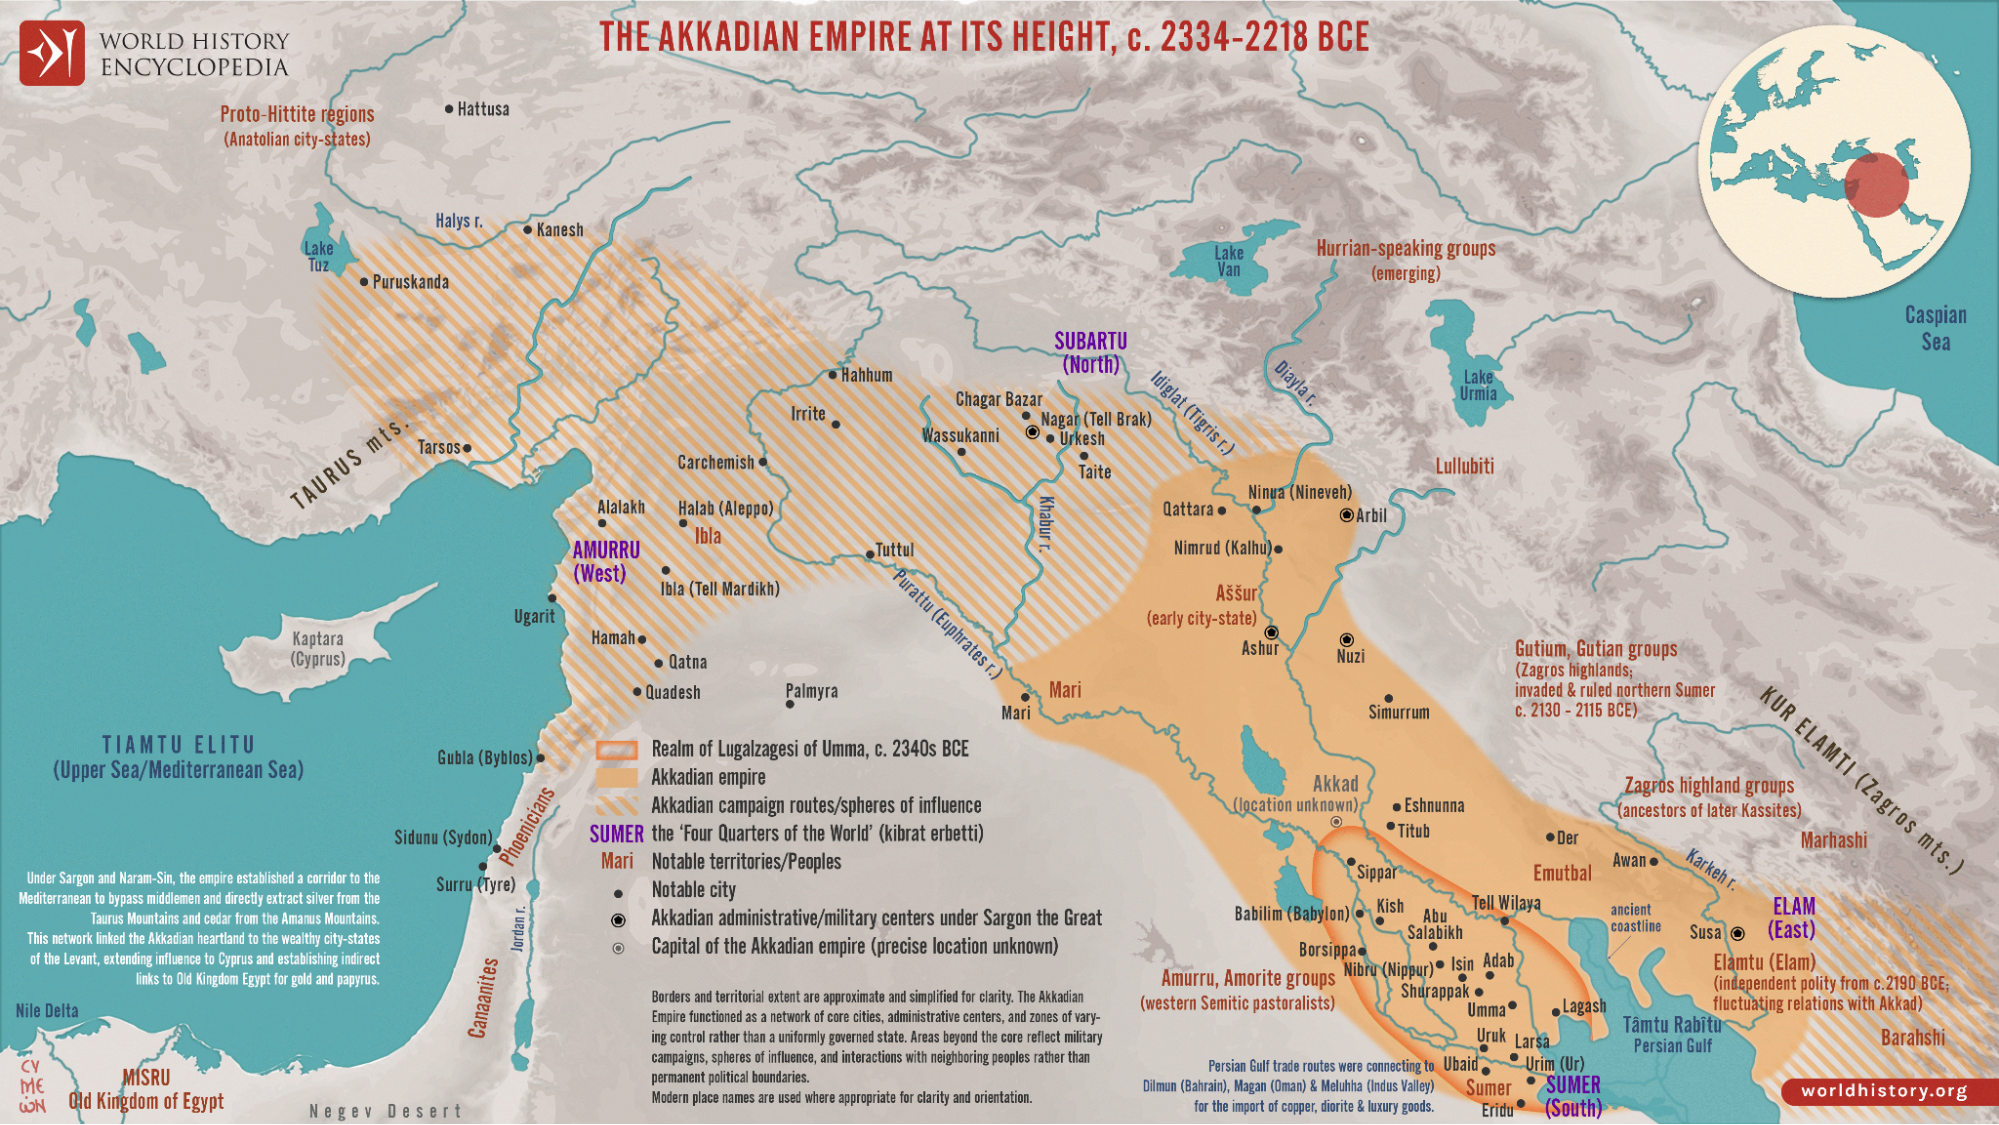
\includegraphics[width=.98\textwidth,height=.52\textheight,keepaspectratio]{image8.png}
\caption{Geographic extent of the Akkadian Empire and major Mesopotamian centers.}\label{fig:12}
\end{figure}

A related problem comes from the cities the tradition associates with Namrud. The book of Genesis, which is the earlier source for much of this material before it was absorbed into Islamic exegetical literature, names Babel, Erech, Akkad, and Calneh as cities in the land of Shinar associated with this figure's kingdom. Erech is generally identified with Uruk, one of the very oldest cities in Mesopotamia, with roots going back to the fourth millennium BCE. Akkad refers to the capital of the Akkadian Empire, founded under Sargon around the twenty-fourth century BCE. Babel, or Babylon, did not become a major political center until considerably later, rising to real prominence under Hammurabi in the eighteenth century BCE and again much later as the capital of the Neo-Babylonian Empire.

These cities were founded, or rose to political importance, across a span of well over a thousand years, not within the lifetime of a single ruler. This creates a real chronological problem for anyone reading the tradition as a literal historical account of one king founding or ruling over all of these places at once. Biblical scholars working on the Genesis text have generally read this passage as a kind of symbolic or summarizing genealogy, a way of representing Mesopotamian civilization and its major centers in a compressed, schematic form, rather than as a precise historical record of one individual's political career. This paper finds this reading reasonably persuasive given the chronological evidence, though it should be said plainly that this is an interpretation of the text's genre and purpose, not something that can be proven the way the mummification evidence in the previous case study can be demonstrated through direct physical examination.

\subsection{The Composite Figure Hypothesis}\label{subsec:5-4}

\begin{figure}[htbp]
\centering
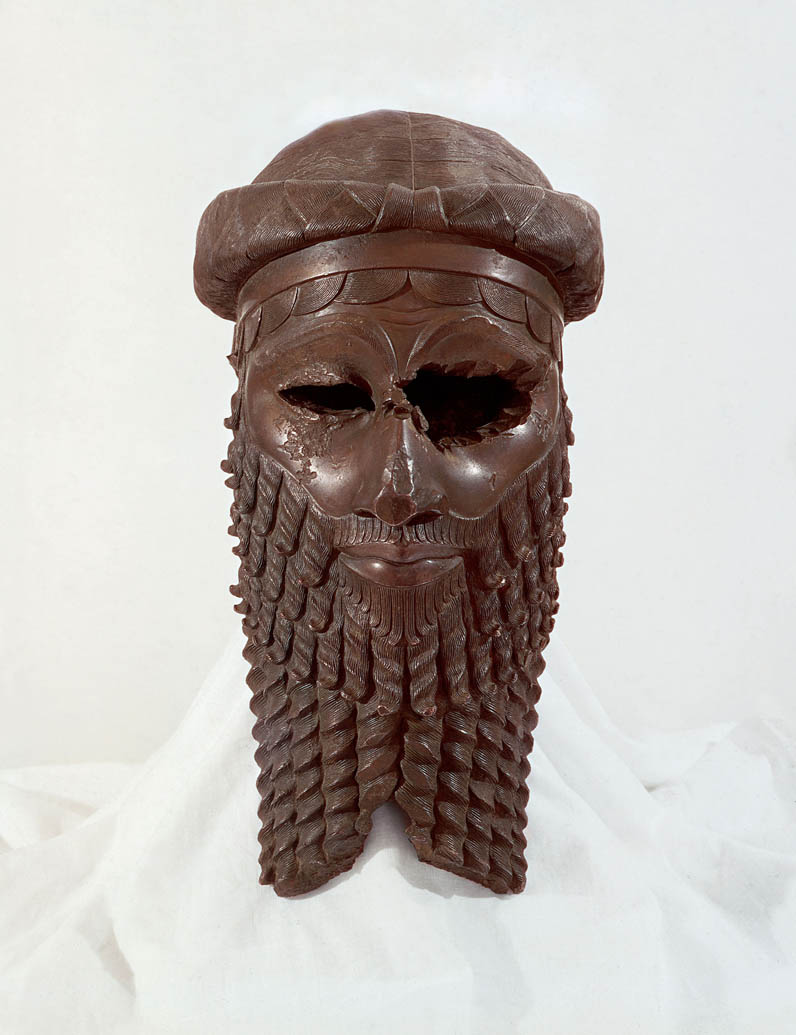
\includegraphics[width=.86\textwidth,height=.31\textheight,keepaspectratio]{image1.png}
\caption{Bronze portrait traditionally associated with Sargon of Akkad.}\label{fig:13}
\end{figure}

Given the absence of Namrud from the native record and the chronological problems with the city list, a number of scholars working in biblical studies and ancient Near Eastern history have proposed that Namrud may not correspond to one historical individual at all, but instead represents a composite figure, built up over a long period of oral and literary transmission from the memory of several real but separate Mesopotamian rulers and traditions.

A few specific candidates come up repeatedly in this scholarship. Sargon of Akkad, the founder of the Akkadian Empire and one of the most legendary conquerors in Mesopotamian memory, is often mentioned, given his association with founding Akkad specifically and his broader reputation in later Mesopotamian literature as a model of ambitious, world spanning kingship. Sargon's grandson, Naram-Sin, is also sometimes mentioned, particularly because of a later Mesopotamian text known as the Curse of Akkad, which describes Naram-Sin committing an act of impiety against the god Enlil that brings divine punishment down on his empire, a theme that has some resemblance to the later Namrud tradition's emphasis on a king brought low by divine judgment for arrogance. A separate line of scholarship has focused on the name itself, noting a possible connection between Namrud or Nimrod and Ninurta, a Mesopotamian war and hunting deity, which would help explain the description of this figure in Genesis as a mighty hunter, an epithet that does not obviously fit a conventional king but fits a divine or semi-divine hunting figure reasonably well.

None of these identifications has anything close to scholarly consensus behind it, and it is worth being honest about that rather than presenting any one of them as settled. They are reasonable hypotheses built on real points of similarity, in name, in theme, or in associated city, between Namrud and specific figures or traditions documented in the native Mesopotamian record. But a hypothesis built on thematic resemblance is a different and weaker kind of claim than a hypothesis built on direct textual identification, and this paper treats it accordingly. What can be said with more confidence is the negative finding from section~\ref{subsec:5-2}, that no single, clearly attested historical ruler named Namrud appears in the primary sources. The positive question of what real history, if any, lies behind the legendary figure remains genuinely open, and reasonable scholars have proposed different answers to it.

\subsection{The Mosquito Death: Origins in Exegetical Literature}\label{subsec:5-5}

\begin{figure}[htbp]
\centering

\includegraphics[width=.86\textwidth,height=.31\textheight,keepaspectratio]{image4.png}
\caption{Nineteenth-century artistic depiction of Nimrod. This image represents later cultural memory rather than historical evidence.}\label{fig:14}
\end{figure}

The death of Namrud by a gnat or mosquito entering his brain is, as noted in section~\ref{subsec:5-1}, part of the later exegetical and storytelling tradition rather than something stated directly in the Quranic text. The story appears in various forms across different commentators and collections of prophetic tales, with details that shift somewhat between versions, including how long the insect tormented him before his death, with some versions giving a period of days and others a much longer symbolic period, and including the detail, found in several versions, that his servants would beat his head with sandals to relieve the pain, which some later folk tradition connects to the origin of certain drumming or head covering customs, though this kind of folk etymology should be treated with real caution.

There is no archaeological or medical evidence that could realistically confirm or disconfirm a story of this kind, and it is worth being direct about why. Unlike the Pharaoh case, where a specific named mummy exists and can be physically examined, Namrud has no surviving body associated with him, no tomb, no skeletal record, nothing that forensic science could examine the way Saleem and Hawass examined the Egyptian royal mummies. The claim is also not the kind of claim that leaves the sort of trace archaeology typically looks for. A death by sudden, undocumented internal causes attributed in later legend to an insect would not necessarily leave any distinguishing mark even if some historical kernel of truth lay behind it. This means the mosquito death story sits in a different evidentiary category from the Pharaoh case discussed in the previous section. It is not so much a claim that has been tested and found wanting under forensic examination. It is a claim that exists almost entirely outside the kind of evidence historical or forensic method requires before it can evaluate anything at all.

This is itself worth noting as a finding, distinct from a verdict on whether the story is true or false. The Pharaoh case involved a specific, falsifiable physical claim, that a particular mummy shows evidence of unexplained preservation following drowning, and that claim could be checked directly against CT data and turned out not to hold up. The Namrud case involves a claim built on a figure who cannot be securely located in the historical record in the first place, attached to a story with no surviving physical referent of any kind. The two cases fail differently. One fails a test it was specific enough to take. The other is not specific enough, in a historical sense, to take the test at all.

\subsection{Comparing the Evidentiary Gap to the Pharaoh Case}\label{subsec:5-6}

It is worth pausing here to compare the two case studies directly, since the comparison says something useful about how these apologetic claims are constructed more generally.

The Pharaoh claim borrows credibility from the fact that mummies are real, physical, examinable objects sitting in a known museum. This gives the claim an appearance of testability that the underlying logic, as section~\ref{sec:4} showed, does not actually deliver, since the connection between the mummy and the unnamed Quranic Pharaoh remains unsupported by the text itself. The Namrud claim works differently. It does not have a physical object to point to at all. Its persuasive force comes instead from the detail and internal consistency of the story as told and retold across centuries of exegetical literature, and from its long standing place within the tradition, rather than from any external, checkable evidence.

Both cases, despite this difference, share the same underlying structure identified in the methodology section. A theological narrative is treated as though it were also a historical record, with a specific named or implied historical referent, when the available evidence, textual, archaeological, or forensic, does not support that referent with anything like the confidence the popular presentation implies. In the Pharaoh case, this is demonstrated through direct forensic contradiction. In the Namrud case, it is demonstrated through the absence of any historical anchor for the figure in the first place, combined with a documented history of the story's gradual development through layers of exegesis and borrowed narrative material, rather than through a single, original historical account.

\subsection{Summary of Findings}\label{subsec:5-7}

Namrud does not appear under that name, or under any clearly corresponding name, in any surviving native Mesopotamian king list, despite those lists being reasonably extensive for the periods in question. The cities later tradition associates with his kingdom, Babel, Erech, Akkad, and Calneh, rose to prominence at different points across more than a thousand years of Mesopotamian history, which creates a serious chronological problem for reading the tradition as a literal account of one ruler's reign. A range of scholars have proposed that Namrud may represent a composite figure, drawing on the memory of historical rulers such as Sargon of Akkad or Naram-Sin, or on the Mesopotamian deity Ninurta, though none of these identifications carries anything close to consensus, and this paper presents them as interpretation rather than established fact. The detailed story of Namrud's death by a gnat or mosquito comes not from the Quran directly but from later tafsir and qisas al-anbiya literature, material that classical Islamic scholarship itself treated with some caution due to its partial origin in borrowed, non-Quranic narrative tradition. This story has no surviving physical evidence of any kind that could be examined, which places it in a fundamentally different evidentiary position than the Pharaoh case, where a specific named mummy exists and could be, and was, directly tested against the claim made about it.

The next section turns to a different kind of case, the death of Abu Jahl at the Battle of Badr, as a point of comparison. Unlike either case examined so far, this is a death reported in early Islamic historical sources without supernatural elements attached to it, and looking at it briefly helps clarify what a more ordinary, historically grounded claim looks like sitting next to the two legendary narratives this paper has spent most of its attention on so far.

\FloatBarrier
\section{Comparative case : Abu Jahl at Badr}\label{sec:6}

\subsection{Why Include This Case}\label{subsec:6-1}

\begin{figure}[htbp]
\centering
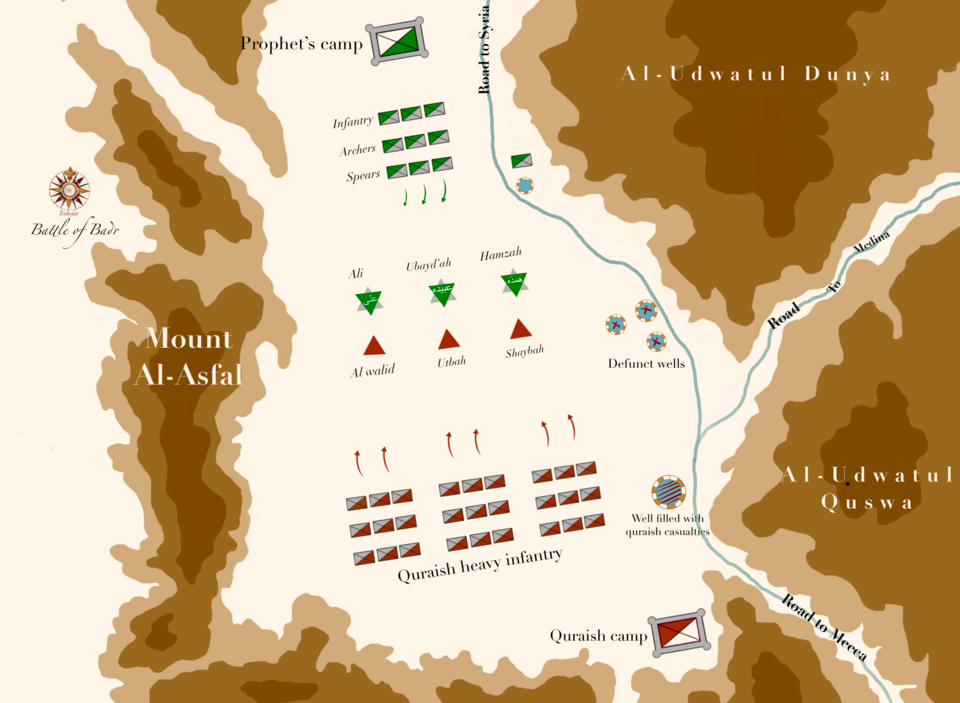
\includegraphics[width=.98\textwidth,height=.52\textheight,keepaspectratio]{image7.png}
\caption{Battlefield layout of Badr, 624 CE.}\label{fig:15}
\end{figure}

The previous two sections looked at claims that turned out to have real evidentiary problems once they were checked closely. It is worth pausing here and looking at a different kind of case, one that comes from inside the same broader literary and religious tradition but does not carry the same problems. The point of this section is not to argue anything new about Abu Jahl himself. It is to show, using an actual example, what a death reported within early Islamic literature looks like when it is not dressed up with supernatural or forensic claims attached to it. This gives the paper something to compare the previous two case studies against, rather than just comparing them to an abstract standard.

Abu Jahl, whose given name was Amr ibn Hisham, was one of the most prominent Meccan opponents of Muhammad in the years before the Hijra, and he remained a leading figure in the Meccan military effort against the early Muslim community afterward. He was killed at the Battle of Badr in 624 CE, the first major military engagement between the Meccans and the Muslims of Medina. His death is reported across multiple early Islamic sources, and it is reported as an ordinary, if notable, battlefield death.

\subsection{The Sources}\label{subsec:6-2}

The main sources for Abu Jahl's death come from two overlapping bodies of early Islamic literature. The first is sira, meaning biography, specifically the biography of Muhammad compiled by Ibn Ishaq in the eighth century and later edited and transmitted by Ibn Hisham, whose recension is the version that survives today. The second is hadith literature, meaning reports of the sayings and actions of Muhammad and his companions, transmitted through chains of named narrators and later collected and evaluated by hadith scholars according to fairly developed methods of source criticism. Accounts of Abu Jahl's death appear in both bodies of material, including in collections regarded as highly reliable within the hadith tradition, such as Sahih al-Bukhari.

It is worth being honest about the limits of this material before describing what it says. Ibn Ishaq was writing more than a century after the events of Badr, working from earlier oral and written material that does not all survive independently for us to check against his version. Hadith scholars developed detailed methods for evaluating the reliability of chains of transmission, distinguishing stronger and weaker reports, and by those internal standards the reports of Abu Jahl's death are generally considered well attested. But this is still a different category of evidence from a CT scan of a physical body. It depends on the reliability of oral transmission and written copying across multiple generations, the same kind of evidence historians work with for most of ancient and early medieval history generally, since physical, directly testable evidence of this kind is the exception rather than the rule for events from this period, in any tradition.

\subsection{What the Sources Report}\label{subsec:6-3}

The core narrative, with some variation in detail between different versions, runs as follows. During the fighting at Badr, Abu Jahl was struck down by two young fighters from the Medinan side, usually identified as Muadh ibn Amr ibn al-Jamuh and Muadh ibn Afra, both still quite young at the time. Accounts differ slightly on exactly how the encounter unfolded and which of the two struck the more serious blow, which is a normal kind of variation to find across independently transmitted battlefield accounts rather than a sign of fabrication. Abu Jahl was left wounded but alive. He was later found on the battlefield by Abdullah ibn Mas'ud, one of Muhammad's companions, who is reported to have confirmed his identity, finished him with a final blow, and removed his head as proof of his death, which was then brought back and shown to Muhammad.

This is, by any reasonable description, a mundane death. It involves sword wounds inflicted during open combat, a wounded man found on a battlefield, and a final killing blow. There is no claim in any of the early sources that his body was preserved in some unusual way, that a natural force intervened directly to kill him, or that any unexplained physical sign was left on or around his body afterward. The sources report what amounts to an ordinary casualty of seventh century warfare, notable mainly because of who Abu Jahl was and the symbolic weight his death carried for the early Muslim community, not because of anything unusual about the death itself.

\subsection{Multiple Attestation}\label{subsec:6-4}

One feature of this case worth highlighting, since it connects directly to the evidentiary standards laid out in the methodology section, is that the core elements of the story, that Abu Jahl was struck down by two young Medinan fighters and finished off by Ibn Mas'ud, appear across more than one line of transmission and more than one type of source, sira material and hadith material, rather than resting on a single unverifiable account. Historians generally treat multiple, semi-independent attestation as a meaningful, if not decisive, point in favor of a report's reliability, since it reduces the chance that the entire account traces back to a single point of invention or error. This does not make the account immune to question. Variation in detail between versions, such as disagreement over exactly which of the two young fighters struck the more disabling blow, shows that the tradition was not perfectly uniform, and a careful historian notes that variation rather than smoothing it away. But the basic shape of the event, an ordinary battlefield death involving named individuals in a named battle, is consistent across the surviving material in a way that the Namrud narrative, discussed in the previous section, is not.

\subsection{The Absence of Supernatural Framing}\label{subsec:6-5}

This is the central point of including this case at all. Nothing about the way Abu Jahl's death is reported in early Islamic sources resembles the structure of the Pharaoh or Namrud claims examined earlier in this paper. No source claims that his body defied natural decay. No source attributes his death to an unusual or unexplained natural mechanism requiring forensic confirmation. No later apologetic literature, as far as this paper is aware, has tried to argue that modern science has proven something extraordinary about how he died. The death is reported, accepted by the historical tradition, and left alone, without being pressed into service as evidence of anything beyond what it plainly is, a man dying in battle.

This matters for the comparison this paper is trying to draw. The methodological problems identified in the Pharaoh and Namrud cases were not problems with religious narrative as such. They were specific problems with a specific kind of claim, where a theological narrative gets reframed as a forensic or historical proof point using evidence that does not actually support that reframing. Abu Jahl's death shows that the same broader textual and historical tradition is fully capable of reporting a death in plain, historically ordinary terms, without that reframing. The issue identified in this paper is not inherent to religious literature in general. It shows up specifically where a narrative is pushed to do evidentiary work it was not built to do.

\subsection{Summary of Findings}\label{subsec:6-6}

Abu Jahl's death at Badr is reported across multiple early Islamic sources, sira and hadith material alike, with the core details reasonably consistent despite some natural variation in specifics. The death itself, sword wounds sustained in battle followed by a final killing blow, is medically and historically unremarkable, and no early source attaches any supernatural or unexplained element to it. This makes it a useful point of contrast against the Pharaoh and Namrud cases, not because it proves anything about those cases directly, but because it shows what an ordinary, historically grounded claim looks like within the same broader tradition, a claim that does not require, and does not receive, the kind of forensic or empirical framing that the previous two case studies depend on and ultimately cannot support. The difference between these cases is not a difference in which religious tradition they come from. It is a difference in what kind of claim is actually being made, and whether that claim asks more of the evidence than the evidence can give.

\FloatBarrier
\section{Discussion}\label{sec:7}

\subsection{What the Two Case Studies Have in Common}\label{subsec:7-1}

Before getting into the more general discussion, it is worth stating plainly what the previous three sections have shown, since the discussion section depends on having that summary clear.

The Pharaoh case and the Namrud case fail in different ways, as section~\ref{subsec:5-6} already pointed out. One fails a specific, testable forensic claim. The other lacks the kind of historical anchor needed to even reach the testing stage. But both cases share a deeper structural similarity, and that similarity is really what this paper has been trying to identify all along. In both cases, a narrative that originates within a theological framework, where its truth depends on revelation and religious authority, gets repackaged as though it were an independently verifiable historical or scientific finding. The Abu Jahl case in section~\ref{sec:6} was included specifically to show that this repackaging is not something that happens automatically whenever a religious tradition reports a death or an event. It happens in particular cases, for particular reasons. The rest of this section tries to think through why.

\subsection{Confirmation Bias and Motivated Reasoning}\label{subsec:7-2}

Confirmation bias is a fairly well established concept in psychology, referring to the tendency people have to notice, accept, and remember evidence that supports something they already believe, while overlooking or dismissing evidence that does not. Motivated reasoning is a related but slightly broader idea, describing the way reasoning itself can be shaped by a desired conclusion, where a person is not consciously lying but is nonetheless working backward from an answer they already want to reach, selecting and interpreting evidence along the way to support it.

Both of these concepts seem relevant to how the Pharaoh claim in particular has been built and sustained over time. Bucaille's original interpretation of the salt residue on Merneptah's mummy is a reasonable example of motivated reasoning in practice. He was not fabricating data. He genuinely found salt on the mummy's skin. But he was already working within a larger project aimed at finding scientific confirmation for Quranic verses, and that prior goal appears to have shaped how he interpreted an ambiguous piece of evidence, salt residue, that had a far more mundane and well documented explanation available, embalming with natron, which he either did not know about or did not give sufficient weight to. A researcher without that prior motivation, encountering salt on an Egyptian mummy, would have little reason to reach first for drowning as an explanation, given how well known the use of natron in embalming already was by the 1970s among specialists in the field.

The pattern repeats, and arguably intensifies, in how the claim has spread since Bucaille. Each subsequent writer or content creator repeating the claim is not independently re-examining the mummy. They are repeating an existing claim that already fits a conclusion they find appealing, and the persuasive packaging, CT scans, forensic language, gets added on top, often without the writer engaging with the actual CT literature in any detail. This is a fairly ordinary pattern in how claims of this kind circulate generally, not unique to this topic or this tradition. A claim that confirms what an audience already wants to believe spreads faster and gets checked less carefully than a claim that does not, regardless of the subject matter.

It is worth being fair here and noting that confirmation bias is not a special failing limited to religious apologetics. It shows up across nearly every kind of motivated argument, political, commercial, and academic included. This paper is not arguing that religious thinkers are uniquely prone to this kind of error. It is arguing that this particular claim, examined closely, shows the pattern clearly, and that noticing the pattern helps explain why the claim has persisted and spread despite the forensic problems laid out in section~\ref{sec:4}.

\subsection{Where Theology and Historiography Diverge}\label{subsec:7-3}

The deeper issue underneath confirmation bias, in this case, is a difference in what theology and historiography are actually trying to do, and what kind of standard each field uses to decide whether a claim should be accepted.

Theology, broadly speaking, often works from a starting position of trust in a particular source of authority, whether that is scripture, tradition, or revelation, and builds outward from there. This is not unreasonable on its own terms. A theological argument can be internally coherent, well reasoned, and intellectually serious while still resting, at its foundation, on an axiom that is accepted on faith rather than proven through external evidence. This is true of religious traditions generally, not just the ones discussed in this paper, and it is also true, in a different form, of certain foundational commitments in other fields, including some assumptions historians themselves rely on without being able to fully prove them from first principles.

Historiography works differently. It does not start from trust in a particular source. It starts from a working assumption of doubt, and sources have to earn credibility through corroboration, internal consistency, and consistency with the wider archaeological and documentary record. A historian reading an ancient text does not begin by assuming it is accurate. They begin by asking what kind of text it is, who wrote it, when, for what purpose, and what other evidence might confirm or complicate what it says. This is a slower and more conditional way of building knowledge, and it often produces conclusions that are tentative, qualified, and open to revision, rather than final and certain.

The problem identified throughout this paper is not that theology uses a faith based standard and historiography uses an evidence based standard. Both of those are legitimate ways of approaching different kinds of questions. The problem is what happens when a claim built on the theological standard gets presented using the language and authority of the historical and scientific standard, without actually being held to that standard. The Pharaoh claim is a theological claim, that God preserved a body as a sign, wearing the clothing of a historical and forensic claim, that a specific named mummy shows physical evidence a scientist would recognize as confirming this. When the claim is examined using the standard it is dressed up in, rather than the standard it actually originates from, it does not hold together. This is not a criticism of theology as a mode of thought. It is a criticism of using theology's conclusions while borrowing historiography's authority, without doing historiography's work.

\subsection{Persuasiveness Is Not the Same as Validity}\label{subsec:7-4}

The final point worth raising here is one that applies beyond this specific paper, though it is illustrated clearly by the cases examined in it. A claim can be highly persuasive to a wide audience while being empirically weak, and a claim can be empirically solid while doing very little to persuade anyone. These two qualities, persuasiveness and validity, are related in everyday reasoning, since people generally expect a true claim to also be the more convincing one, but they are not the same thing, and they do not always move together.

The Pharaoh claim is, by any reasonable measure, persuasive. It uses vivid, concrete imagery, an actual mummy, a real museum, real scientific sounding terminology. It offers a satisfying resolution, where ancient scripture and modern science appear to confirm each other. It is easy to repeat in a short video and easy to share. None of these features have anything to do with whether the claim is actually supported by the forensic literature it claims to draw on. A claim can have all of these persuasive features and still be wrong, in the fairly specific and checkable sense this paper has tried to demonstrate, where the actual CT findings and the actual chemistry of natron point in a different direction than the claim asserts.

This gap between persuasiveness and validity is worth naming directly, because it explains something about why criticism from specialists, Egyptologists pointing out the natron problem since shortly after Bucaille's book appeared, has done relatively little to slow the claim's spread in popular and online religious discourse. Specialist criticism is usually less vivid, less emotionally satisfying, and less shareable than the original claim. A paper correcting a chemistry error does not compete well, in terms of attention, with a short video showing a mummy and announcing that science has confirmed scripture. This is not a new problem, and it is not unique to this topic. It shows up anywhere a simple, satisfying claim competes against a more accurate but less exciting correction, across many fields entirely unrelated to religion.

What this means for the present paper is mostly a matter of expectation management regarding its own argument. Demonstrating, as section~\ref{sec:4} tried to do, that the forensic evidence does not support the Pharaoh claim is not the same thing as expecting that demonstration to be persuasive to everyone who currently finds the original claim compelling. Persuasiveness depends on factors beyond the strength of an argument, including how the argument is presented, what the audience already wants to believe, and how the claim fits into a broader emotional or community context. This paper's goal, as stated in the introduction, was narrower than persuasion. It was to test whether a specific empirical claim holds up against the available evidence, using a fixed and openly stated standard. Whether or not that test result changes anyone's mind is a separate question, and one this paper does not have the tools to answer.

\subsection{Summary}\label{subsec:7-5}

The Pharaoh and Namrud cases both show a pattern where a theological narrative is presented using the language and authority of historical and forensic proof, without actually meeting the standards that language implies. Confirmation bias and motivated reasoning offer a partial explanation for how claims like this get constructed and why they spread, particularly when an investigator or audience already has a strong prior reason to want the claim to be true. A deeper explanation lies in the difference between theology's evidentiary standard, which can reasonably rest on faith and authority, and historiography's evidentiary standard, which requires external corroboration, and in what happens when conclusions reached under the first standard get marketed using the second. Finally, the persuasive power of a claim and its empirical validity are separate qualities that do not necessarily move together, which helps explain why forensic correction of this claim, available in the academic literature for decades, has not significantly slowed its popular spread. None of this amounts to a judgment on the underlying religious tradition itself. It is a judgment, specific and limited, on what happens when a particular kind of evidence gets asked to do work it cannot do.

\FloatBarrier
\section{Conclusion}\label{sec:8}

\subsection{Restating the Three Failures}\label{subsec:8-1}

This paper set out to test a fairly narrow question. Not whether the Exodus account or the Namrud narrative are true in a religious sense, since that question sits outside what historical method can answer, but whether the specific empirical claims built around these narratives, the claims presented online as forensic and scientific proof, actually hold up against the kind of evidence historians and forensic scientists normally require. Three separate problems came up across the case studies, and it is worth restating them together here, since they reinforce each other rather than standing as three unrelated objections.

The first problem was logical. The Quran does not name the Pharaoh of the Exodus, give his dynasty, or provide any detail that would let a historian connect the verse to one specific ruler out of the many who held that title across three thousand years of Egyptian history. Identifying a particular mummy as the Pharaoh in question, something apologists themselves have not even agreed on, requires supplying information the text does not contain, and then treating the resulting match as though it confirmed the verse rather than simply being made to fit it. This is the error described in the methodology section as affirming the consequent, combined with the undistributed middle, where a general title gets quietly treated as though it referred to one verifiable individual.

The second problem was statistical, or really a problem of expectation. A preserved Pharaoh is not a surprising find. Egyptian mummification was a routine, highly developed, state supported practice carried out for roughly three millennia, and dozens of royal mummies with no connection to any Exodus narrative have survived to the present day. Finding one more preserved Pharaoh does not clear the bar the Baseline Expectation Rule sets for treating an observation as evidence of something extraordinary. It is closer to the default outcome of how Egyptian royalty were buried, not an anomaly that calls out for a special explanation.

The third problem was forensic, and this is where the paper spent most of its attention, since it is the most specific and most directly testable of the three. CT and paleoradiological work by researchers such as Sahar Saleem and Zahi Hawass shows mummification consistent with standard Egyptian embalming practice, including evisceration, brain removal through the nasal cavity, and natron packing, rather than any preservation process science cannot account for. The salt residue central to Bucaille's original 1976 claim is well explained by natron, the documented embalming agent, rather than seawater. The advanced age and degenerative disease reported for Ramesses II do not establish his immediate cause of death. Post-mortem damage documented in other royal mummies must be assessed specimen by specimen and cannot simply be transferred to his case. The Namrud case showed a related but distinct kind of forensic gap, not a claim that fails physical testing but a claim that has no physical referent available to test in the first place, with no surviving body, no tomb, and no archaeological trace connecting the legendary figure to any specific historical individual.

\subsection{What the Comparison Case Showed}\label{subsec:8-2}

The Abu Jahl case in section~\ref{sec:6} was included to make sure this paper was not simply assuming that religious historical narrative is unreliable as a category. It is not. Abu Jahl's death at Badr is reported across multiple early Islamic sources, sira and hadith material together, with reasonably consistent core details and no supernatural or forensic claims attached to it at all. This matters for how the paper's overall argument should be read. The problems identified in the Pharaoh and Namrud cases are not problems with religious literature in general. They are specific to what happens when a theological narrative gets reframed as an externally verifiable historical or scientific proof, using evidence that was never built to carry that weight. The same broader tradition that produced the Pharaoh and Namrud claims also produced a plain, historically ordinary account of a death in battle, with no need for any of that reframing.

\subsection{Final Framing}\label{subsec:8-3}

Taken together, these three failures point toward a single underlying conclusion, one that this paper has tried to reach carefully rather than assume from the start. The claims examined in this paper, that a specific mummy provides forensic proof of the Exodus Pharaoh's death by drowning, and that the death of Namrud is a documented historical event rather than a legendary or composite tradition, do not meet the standards historians and forensic scientists normally apply before accepting a claim of this kind. The textual evidence does not support the specific identifications involved. The statistical baseline does not support treating the underlying observations as unusual. The forensic evidence, where it exists at all, points in a different direction than the claim asserts, and where it does not exist, as in the Namrud case, the claim cannot be meaningfully tested either way.

This does not mean these narratives are without value or meaning. It means something narrower and more specific. As historical or forensic claims, claims that assert something checkable about the physical past, they do not hold up. As theological claims, claims about divine action, divine justice, and the meaning of these stories within a framework of religious faith, they remain exactly what they have always been within that framework, matters that depend on revelation and belief rather than external verification. A person can continue to hold these narratives as true in a religious sense without needing them to also be true in a forensic sense, since these are different kinds of claims requiring different kinds of support. What this paper has argued against is not the religious narrative itself, but the practice of presenting that narrative as though it had already passed a scientific test it has, in fact, failed, or in the Namrud case, a test it was never specific enough to take in the first place.

This is, in the end, a fairly modest conclusion, and it is worth ending on that note rather than overstating it. This paper has not disproven the Exodus account or the Namrud tradition as matters of faith, and it was never positioned to do so. What it has shown is that two specific, popular, internet-circulated claims about physical, checkable evidence do not survive contact with the actual textual, archaeological, and forensic record. That is a narrower finding than a full verdict on the truth of these traditions, but it is also, this paper would argue, the only kind of finding historical method was ever equipped to produce.

\FloatBarrier
\section{Bibliography}\label{sec:9}

\subsection*{Forensic and Archaeological Sources (Case Study 1)}

\noindent Saleem, Sahar N., and Zahi Hawass. ``Digital Unwrapping of the Mummy of King Amenhotep I (1525--1504 BC) Using CT.'' Frontiers in Medicine 8 (2021): 778498. \url{https://doi.org/10.3389/fmed.2021.778498}.

\begin{list}{}{\setlength{\leftmargin}{1.5em}\setlength{\itemindent}{-1.5em}}
\item Hawass, Zahi, and Sahar N. Saleem. Scanning the Pharaohs: CT Imaging of the New Kingdom Royal Mummies . Cairo and New York: The American University in Cairo Press, 2016.
\item Wilkinson, Caroline M., Sahar N. Saleem, Ching Yiu Jessica Liu, and Mark Roughley. ``Revealing the Face of Ramesses II through Computed Tomography, Digital 3D Facial Reconstruction and Computer-Generated Imagery.'' Journal of Archaeological Science 160 (2023): 105884. \url{https://doi.org/10.1016/j.jas.2023.105884}.
\end{list}

\subsection*{Bucaille and Bucailism (Case Study 1)}

\begin{list}{}{\setlength{\leftmargin}{1.5em}\setlength{\itemindent}{-1.5em}}
\item Bucaille, Maurice. The Bible, the Qur'an and Science . Paris: Seghers, 1976. English translation, Indianapolis: American Trust Publications, 1978.
\item Bigliardi, Stefano. ``Snakes from Staves? Science, Scriptures and the Supernatural in Maurice Bucaille.'' Zygon: Journal of Religion and Science 46, no. 4 (2011): 793--805.
\item Bigliardi, Stefano. ``The 'Scientific Miracle of the Qur'\={a}n,' Pseudoscience, and Conspiracism.'' Zygon: Journal of Religion and Science 52, no. 1 (2017): 146--171. \url{https://doi.org/10.1111/zygo.12321}.
\item Edis, Taner. An Illusion of Harmony: Science and Religion in Islam . Amherst, NY: Prometheus Books, 2007.
\end{list}

\subsection*{Mesopotamian Sources (Case Study 2)}

\begin{list}{}{\setlength{\leftmargin}{1.5em}\setlength{\itemindent}{-1.5em}}
\item Jacobsen, Thorkild. The Sumerian King List . Assyriological Studies 11. Chicago: University of Chicago Press, 1939.
\item Levin, Yigal. ``Nimrod the Mighty, King of Kish, King of Sumer and Akkad.'' Vetus Testamentum 52, no. 3 (2002): 350--366. \url{https://doi.org/10.1163/156853302760197494}.
\item Van De Mieroop, Marc. A History of the Ancient Near East, ca. 3000--323 BC . 3rd ed. Chichester, UK, and Malden, MA: Wiley-Blackwell, 2016.
\end{list}

\subsection*{Early Islamic Sources (Case Study 3 / Abu Jahl)}

\begin{list}{}{\setlength{\leftmargin}{1.5em}\setlength{\itemindent}{-1.5em}}
\item Ibn Ishaq, Muhammad. The Life of Muhammad: A Translation of Ibn Ishaq's Sirat Rasul Allah . Translated by Alfred Guillaume. Oxford: Oxford University Press, 1955.
\item Sahih al-Bukhari . Multiple standard editions exist; this paper relies on the commonly cited English translation by Muhammad Muhsin Khan.
\end{list}

\subsection*{Primary Religious Texts}

\begin{list}{}{\setlength{\leftmargin}{1.5em}\setlength{\itemindent}{-1.5em}}
\item The Qur'an . Translated by M. A. S. Abdel Haleem. Oxford: Oxford World's Classics, 2004.
\item The Holy Bible (Genesis, for the Namrud/Nimrod material). Any standard critical edition, e.g., the New Revised Standard Version.
\end{list}

\FloatBarrier
\section*{Figure sources}
The two CT figures reproduce figures 2 and 3 of Saleem and Hawass (2021), cited above, under the article's Creative Commons Attribution licence. The remaining illustrations were supplied with the manuscript. Original source and licence details for those files were not included; their reproduction here does not establish provenance or evidential status. The mummification-process diagram bears the Twinkl name. The Akkadian Empire map bears the World History Encyclopedia name. Illustrations and later artistic reconstructions are kept separate from evidence about specific individuals.

\end{document}
